% Latex header for doxygen 1.8.9.1
\documentclass[twoside]{book}

% Packages required by doxygen
\usepackage{fixltx2e}
\usepackage{calc}
\usepackage{doxygen}
\usepackage[export]{adjustbox} % also loads graphicx
\usepackage{graphicx}
\usepackage[utf8]{inputenc}
\usepackage{makeidx}
\usepackage{multicol}
\usepackage{multirow}
\PassOptionsToPackage{warn}{textcomp}
\usepackage{textcomp}
\usepackage[nointegrals]{wasysym}
\usepackage[table]{xcolor}

% Font selection
\usepackage[T1]{fontenc}
\usepackage[scaled=.90]{helvet}
\usepackage{courier}
\usepackage{amssymb}
\usepackage{sectsty}
\renewcommand{\familydefault}{\sfdefault}
\allsectionsfont{%
  \fontseries{bc}\selectfont%
  \color{darkgray}%
}
\renewcommand{\DoxyLabelFont}{%
  \fontseries{bc}\selectfont%
  \color{darkgray}%
}
\newcommand{\+}{\discretionary{\mbox{\scriptsize$\hookleftarrow$}}{}{}}

% Page & text layout
\usepackage{geometry}
\geometry{%
  a4paper,%
  top=2.5cm,%
  bottom=2.5cm,%
  left=2.5cm,%
  right=2.5cm%
}
\usepackage[T1]{fontenc}
\usepackage{titlesec, blindtext, color}
\definecolor{gray75}{gray}{0.75}
\newcommand{\hsp}{\hspace{20pt}}
\titleformat{\chapter}[hang]{\Huge\bfseries}{\thechapter\hsp\textcolor{gray75}{|}\hsp}{0pt}{\Huge\bfseries}
\tolerance=750
\hfuzz=15pt
\hbadness=750
\setlength{\emergencystretch}{15pt}
\setlength{\parindent}{0cm}
\setlength{\parskip}{0.2cm}
\makeatletter
\renewcommand{\paragraph}{%
  \@startsection{paragraph}{4}{0ex}{-1.0ex}{1.0ex}{%
    \normalfont\normalsize\bfseries\SS@parafont%
  }%
}
\renewcommand{\subparagraph}{%
  \@startsection{subparagraph}{5}{0ex}{-1.0ex}{1.0ex}{%
    \normalfont\normalsize\bfseries\SS@subparafont%
  }%
}
\makeatother

% Headers & footers
\usepackage{fancyhdr}
\pagestyle{fancyplain}
\fancyhead[LE]{\fancyplain{}{\bfseries\thepage}}
\fancyhead[CE]{\fancyplain{}{}}
\fancyhead[RE]{\fancyplain{}{\bfseries\leftmark}}
\fancyhead[LO]{\fancyplain{}{\bfseries\rightmark}}
\fancyhead[CO]{\fancyplain{}{}}
\fancyhead[RO]{\fancyplain{}{\bfseries\thepage}}
\fancyfoot[LE]{\fancyplain{}{}}
\fancyfoot[CE]{\fancyplain{}{}}
\fancyfoot[RE]{\fancyplain{}{\bfseries\scriptsize Generated by Yu Chen }}
\fancyfoot[LO]{\fancyplain{}{\bfseries\scriptsize Generated by Yu Chen }}
\fancyfoot[CO]{\fancyplain{}{}}
\fancyfoot[RO]{\fancyplain{}{}}
\renewcommand{\footrulewidth}{0.4pt}
\renewcommand{\chaptermark}[1]{%
  \markboth{#1}{}%
}
\renewcommand{\sectionmark}[1]{%
  \markright{\thesection\ #1}%
}

% Indices & bibliography
\usepackage{natbib}
\usepackage[titles]{tocloft}
\setcounter{tocdepth}{3}
\setcounter{secnumdepth}{5}
\makeindex

% Hyperlinks (required, but should be loaded last)
\usepackage{ifpdf}
\ifpdf
  \usepackage[pdftex,pagebackref=true]{hyperref}
\else
  \usepackage[ps2pdf,pagebackref=true]{hyperref}
\fi
\hypersetup{%
  colorlinks=true,%
  linkcolor=blue,%
  citecolor=blue,%
  unicode%
}

% Custom commands
\newcommand{\clearemptydoublepage}{%
  \newpage{\pagestyle{empty}\cleardoublepage}%
}


%===== C O N T E N T S =====

\usepackage[yyyymmdd,hhmmss]{datetime}

\begin{document}

% Titlepage & ToC
\hypersetup{pageanchor=false,
             bookmarks=true,
             bookmarksnumbered=true,
             pdfencoding=unicode
            }
\pagenumbering{roman}
\begin{titlepage}
\vspace*{7cm}
\begin{center}%
{\Huge Dual State Framework}\\
\vspace*{0.5cm}
{\Large API Document}\\
\vspace*{1cm}
{\normalsize Yu Chen - C00151352}\\
\vspace*{0.2cm}
{\small \today\ \currenttime}\\
\end{center}
\end{titlepage}
\clearemptydoublepage
\tableofcontents
\clearemptydoublepage
\pagenumbering{arabic}
\hypersetup{pageanchor=true}

%--- Begin generated contents ---
\chapter{Get Started}
\label{index}\hypertarget{index}{}\hypertarget{index_welcome}{}\section{Welcome}\label{index_welcome}
Welcome to the official D\+S\+F documentation. Here you will find a detailed view of all the D\+S\+F classes and functions. If you have not installed D\+S\+F, you may be interested in how to install D\+S\+F on \hyperlink{_mac}{Mac os X }, \hyperlink{_win}{M\+S Windows }, and \hyperlink{_linux}{Linux }.\hypertarget{index_example}{}\section{Short example}\label{index_example}
Here is a short example, to show you how simple it is to use D\+S\+F\+: \hypertarget{index_dsf}{}\subsection{Implementing Dual\+State\+Framework}\label{index_dsf}
My\+D\+S\+F.\+h 
\begin{DoxyCodeInclude}
\textcolor{preprocessor}{#ifndef \_\_DSFExample\_\_MyDSF\_\_}
\textcolor{preprocessor}{#define \_\_DSFExample\_\_MyDSF\_\_}

\textcolor{preprocessor}{#include <\hyperlink{_dual_state_framework_8h}{dsf/DualStateFramework.h}>}

\textcolor{keyword}{class }MyDSF : \textcolor{keyword}{public} \hyperlink{classdsf_1_1_dual_state_framework}{dsf::DualStateFramework} \textcolor{comment}{// Extends dsf::DualStateFramework}
\{
\textcolor{keyword}{public}:
    \textcolor{keyword}{explicit} MyDSF() : \hyperlink{namespacedsf_a68ac3b6a0526bfa7f6a412918afb1841}{DualStateFramework}() \{\} \textcolor{comment}{// Uses default super constructor}
    \textcolor{keywordtype}{void} \hyperlink{classdsf_1_1_dual_state_framework_a809a7bba4148e17ea9a43a0a035383ba}{initialize}()\textcolor{keyword}{ override }\{\}
\};

\textcolor{preprocessor}{#endif}
\end{DoxyCodeInclude}
\hypertarget{index_syncObj}{}\subsection{Implementing dsf\+::\+Synchronized\+Object}\label{index_syncObj}
Sync\+Obj.\+h 
\begin{DoxyCodeInclude}
\textcolor{preprocessor}{#ifndef DSFExample\_SyncObj\_h}
\textcolor{preprocessor}{#define DSFExample\_SyncObj\_h}

\textcolor{preprocessor}{#include <\hyperlink{_synchronized_object_8h}{dsf/SynchronizedObject.h}>}

\textcolor{keyword}{class }SyncObj : \textcolor{keyword}{public} \hyperlink{classdsf_1_1_synchronized_object}{dsf::SynchronizedObject} \textcolor{comment}{// Extends dsf::SynchronizedObject}
\{
\textcolor{keyword}{public}:
    SyncObj(\textcolor{keywordtype}{int} v) : \hyperlink{namespacedsf_acbf1798fc56cfb1707162a17e13f5fda}{SynchronizedObject}(), v(v) \{\} \textcolor{comment}{// Uses default super constructor}
    \textcolor{keywordtype}{int} getValue() \{
        \textcolor{keywordflow}{return} this->v;
    \}
\textcolor{keyword}{protected}:
    \textcolor{keywordtype}{void} \hyperlink{classdsf_1_1_synchronized_object_ae94875bd63d8071f8a563ac45ca7ccc2}{run}()\textcolor{keyword}{ override }\{ \textcolor{comment}{// Overrides pure virtual function}
        \textcolor{keywordflow}{if}(this->\hyperlink{classdsf_1_1_synchronized_object_a3ce496c6aaecc4b0ca3a4d09539a4920}{receive}()) \textcolor{comment}{// Returns the number of message received}
            this->\hyperlink{classdsf_1_1_task_box_ad35070ac305146aaa4073b2078d9209e}{process}(); \textcolor{comment}{// Executes received messages}
    \}
\textcolor{keyword}{private}:
    \textcolor{keywordtype}{int} v;
\};

\textcolor{preprocessor}{#endif}
\end{DoxyCodeInclude}
\hypertarget{index_manager}{}\subsection{Creating a manager class}\label{index_manager}
Obj\+Manager.\+h 
\begin{DoxyCodeInclude}
\textcolor{preprocessor}{#ifndef DSFExample\_ObjManager\_h}
\textcolor{preprocessor}{#define DSFExample\_ObjManager\_h}

\textcolor{preprocessor}{#include "MyDSF.h"}
\textcolor{preprocessor}{#include "SyncObj.h"}
\textcolor{preprocessor}{#include <iostream>}

\textcolor{keyword}{class }ObjManager
\{
\textcolor{keyword}{public}:
    MyDSF* dsf;
    \hyperlink{namespacedsf_aa16e735f29587f4485b56fc46746f7a9}{dsf::TaskFunction}* print;
    
    ObjManager(MyDSF* dsf) : dsf(dsf) \{  \textcolor{comment}{// Alias DSF pointer}
        \textcolor{comment}{// Initialises TaskFunctions}
        this->print = \textcolor{keyword}{new} \hyperlink{namespacedsf_aa16e735f29587f4485b56fc46746f7a9}{dsf::TaskFunction}([\textcolor{keyword}{this}](
      \hyperlink{classdsf_1_1_synchronized_object}{dsf::SynchronizedObject}* to,
                                                   \hyperlink{classdsf_1_1_synchronized_object}{dsf::SynchronizedObject}* from,
                                                   \hyperlink{namespacedsf_abe4bf68433935a81c31a5ada9b17663a}{dsf::TaskArgument}* args)
                                               \{
                                                   \textcolor{keyword}{auto} syncObj = args->to<SyncObj*>();
                                                   std::cout << syncObj->getValue();
                                                   this->dsf->remove(to);
                                               \});

    \}
    ~ObjManager() \{
        \textcolor{keyword}{delete} this->print;
    \}
\};

\textcolor{preprocessor}{#endif}
\end{DoxyCodeInclude}
\hypertarget{index_main}{}\subsection{Running D\+S\+F}\label{index_main}
main.\+cpp 
\begin{DoxyCodeInclude}
\textcolor{preprocessor}{#include "MyDSF.h"}
\textcolor{preprocessor}{#include "SyncObj.h"}
\textcolor{preprocessor}{#include "ObjManager.h"}

\textcolor{keywordtype}{int} main(\textcolor{keywordtype}{int} argc, \textcolor{keyword}{const} \textcolor{keywordtype}{char} * argv[]) \{
    \textcolor{keyword}{const} \textcolor{keywordtype}{int} NUMBER\_OF\_OBJS = 100;
    \textcolor{keyword}{auto} dsf = \textcolor{keyword}{new} MyDSF();
    \textcolor{keyword}{auto} om = \textcolor{keyword}{new} ObjManager(dsf);
    SyncObj* sos[NUMBER\_OF\_OBJS];
    \textcolor{keywordflow}{for}(\textcolor{keywordtype}{int} i = 0; i < NUMBER\_OF\_OBJS; i ++) \{ \textcolor{comment}{// Creates NUMBER\_OF\_OBJS SyncObj objects}
        sos[i] = \textcolor{keyword}{new} SyncObj(i);
        dsf->add(sos[i]); \textcolor{comment}{// Adds objects to DSF object}
        dsf->send(sos[i], sos[i], om->print, \textcolor{keyword}{new} \hyperlink{namespacedsf_abe4bf68433935a81c31a5ada9b17663a}{dsf::TaskArgument}(sos[i])); \textcolor{comment}{// Sends
       messages}
    \}
    dsf->start();
    \textcolor{keyword}{delete} dsf;
    \textcolor{keyword}{delete} om;
    \textcolor{keywordflow}{return} 0;
\}
\end{DoxyCodeInclude}
 
\chapter{Installation}
\label{_installation}
\hypertarget{_installation}{}
Dual State Framework uses \hyperlink{}{yctools } and \hyperlink{}{Intel tbb }. Before the installation you need to install them first.\hypertarget{_installation_Mac}{}\section{Mac O\+S X}\label{_installation_Mac}
\hypertarget{_installation_dependencies_mac}{}\subsection{Install Dependencies}\label{_installation_dependencies_mac}
\begin{DoxyParagraph}{yctools}
Download\+: \hyperlink{}{\href{https://sourceforge.net/projects/yctools/}{\tt https\+://sourceforge.\+net/projects/yctools/} } ~\newline
 Download the pkg file and install it.
\end{DoxyParagraph}
\begin{DoxyParagraph}{Intel tbb}
Download\+: \hyperlink{}{\href{https://www.threadingbuildingblocks.org/download}{\tt https\+://www.\+threadingbuildingblocks.\+org/download} } ~\newline
 Download the O\+S X version and unzip it. ~\newline
 Inside the directory, copy \char`\"{}libtbb.\+dylib\char`\"{} in the subdirectory \char`\"{}lib\char`\"{} to \char`\"{}/usr/lib\char`\"{} or \char`\"{}/usr/local/lib\char`\"{}. ~\newline
 Next, copy the directory \char`\"{}include/dsf\char`\"{} to \char`\"{}/usr/include\char`\"{} or \char`\"{}/usr/local/include\char`\"{}.
\end{DoxyParagraph}
\hypertarget{_installation_dsf_mac}{}\subsection{Install Dual State Framework}\label{_installation_dsf_mac}
Download\+: \hyperlink{}{\href{https://sourceforge.net/projects/dualstateframework/}{\tt https\+://sourceforge.\+net/projects/dualstateframework/} } ~\newline
 Download the pkg file and install it.\hypertarget{_installation_use_mac}{}\subsection{Use D\+S\+F in Xcode}\label{_installation_use_mac}
To use this framework in Xcode is very simple. You just need to drag dsf.\+framework and yctools.\+framework to your project explorer.\hypertarget{_installation_Win}{}\section{Microsoft Windows}\label{_installation_Win}
\hypertarget{_installation_dependencies_win}{}\subsection{Install Dependencies}\label{_installation_dependencies_win}
\begin{DoxyParagraph}{yctools}
Download\+: \hyperlink{}{\href{https://sourceforge.net/projects/yctools/}{\tt https\+://sourceforge.\+net/projects/yctools/} } ~\newline
 Download the exe file and install it. ~\newline
 The installation will create an environment variable \char`\"{}yctools\char`\"{} which refers to the program installed path.
\end{DoxyParagraph}
\begin{DoxyParagraph}{Intel tbb}
Download\+: \hyperlink{}{\href{https://www.threadingbuildingblocks.org/download}{\tt https\+://www.\+threadingbuildingblocks.\+org/download} } ~\newline
 Download the Window O\+S version and unzip it. ~\newline
 Inside the directory, copy \char`\"{}tbb.\+lib\char`\"{} in the subdirectory \char`\"{}lib/your architecture/your visual studio version\char`\"{} to \char`\"{}where you want to store them/lib\char`\"{}. ~\newline
 Copy \char`\"{}tbb.\+dll\char`\"{} in the subderectory \char`\"{}bin/your architecture/your visual studio version\char`\"{} to \char`\"{}where you want to store them/bin\char`\"{}. ~\newline
 Add an environment variable \char`\"{}tbb\char`\"{}, and set its value to \char`\"{}where you want to store them\char`\"{}. ~\newline
 Next, copy the directory \char`\"{}include/dsf\char`\"{} to \char`\"{}where you want to store them/include\char`\"{}. 
\end{DoxyParagraph}
\hypertarget{_installation_dsf_win}{}\subsection{Install Dual State Framework}\label{_installation_dsf_win}
Download\+: \hyperlink{}{\href{https://sourceforge.net/projects/dualstateframework/}{\tt https\+://sourceforge.\+net/projects/dualstateframework/} } ~\newline
 Download the exe file and install it. ~\newline
 The installation will create an environment variable \char`\"{}dsf\char`\"{} which refers to the program installed path.\hypertarget{_installation_use_win}{}\subsection{Use D\+S\+F in Visual Studio}\label{_installation_use_win}
\begin{DoxyParagraph}{Add additional header path}
In project properties -\/$>$ C/\+C++ -\/$>$ General -\/$>$ Additional Include Directories, add \$(yctools)\textbackslash{}include, \$(dsf)\textbackslash{}include, and \$(tbb)\textbackslash{}include.
\end{DoxyParagraph}
\begin{DoxyParagraph}{Add Dependencies}
In project properties -\/$>$ Linker -\/$>$ General -\/$>$ Additional Library Directories, add \$(yctools)\textbackslash{}lib, \$(dsf)\textbackslash{}lib, and \$(tbb)\textbackslash{}lib. ~\newline
 In project properties -\/$>$ Linker -\/$>$ Input -\/$>$ Additional Dependencies, add yctools.\+lib, tbb.\+lib, and dsf.\+lib.
\end{DoxyParagraph}
\hypertarget{_installation_Linux}{}\section{Linux}\label{_installation_Linux}
This page is only for Linux with Debian package management tools (Debian, ubuntu, and etc.). Other Linux users please visit \hyperlink{_installation_source}{Compile source code }. \hypertarget{_installation_dependencies_linux}{}\subsection{Install Dependencies}\label{_installation_dependencies_linux}
\begin{DoxyParagraph}{yctools}
Download\+: \hyperlink{}{\href{https://sourceforge.net/projects/yctools/}{\tt https\+://sourceforge.\+net/projects/yctools/} } ~\newline
 Download the deb file and install it.
\end{DoxyParagraph}
\begin{DoxyParagraph}{Intel tbb}
In terminal or console, type 
\begin{DoxyCode}
$ sudo apt-\textcolor{keyword}{get} install libtbb2
\end{DoxyCode}

\end{DoxyParagraph}
\hypertarget{_installation_dsf_linux}{}\subsection{Install Dual State Framework}\label{_installation_dsf_linux}
Download\+: \hyperlink{}{\href{https://sourceforge.net/projects/dualstateframework/}{\tt https\+://sourceforge.\+net/projects/dualstateframework/} } ~\newline
 Download the deb file and install it.\hypertarget{_installation_source}{}\section{Compile source code}\label{_installation_source}
To compile the code, you need a C++ compiler with c++11 supported, git, and C\+Make.\hypertarget{_installation_pre_source}{}\subsection{Pre-\/\+Build}\label{_installation_pre_source}
\begin{DoxyParagraph}{Get source code}

\begin{DoxyCode}
$ git clone https:\textcolor{comment}{//github.com/kuyoonjo/DualStateFramework.git}
\end{DoxyCode}
 
\end{DoxyParagraph}
\begin{DoxyParagraph}{Generate project for compiler}
G\+U\+I version of C\+Make is recommended to generate the project. For more information about cmake, please visit \hyperlink{}{\href{http://www.cmake.org}{\tt http\+://www.\+cmake.\+org} }.
\end{DoxyParagraph}
\hypertarget{_installation_compile_source}{}\subsection{Build the project}\label{_installation_compile_source}
If you generate an Xcode, Visual Studio, or any other G\+U\+I I\+D\+E project, just open the project and build it. ~\newline
 If you generate a Makefile project, in a terminal or console, type 
\begin{DoxyCode}
$ cd \textcolor{stringliteral}{"your project directory"}
$ make
\end{DoxyCode}
 Good luck! 
\chapter{Namespace Documentation}
\hypertarget{namespacedsf}{}\section{dsf Namespace Reference}
\label{namespacedsf}\index{dsf@{dsf}}
\subsection*{Classes}
\begin{DoxyCompactItemize}
\item 
class \hyperlink{classdsf_1_1_dual_state_framework}{Dual\+State\+Framework}
\begin{DoxyCompactList}\small\item\em The starting pointer for the framework is the abstract class \hyperlink{classdsf_1_1_dual_state_framework}{dsf\+::\+Dual\+State\+Framework}. \end{DoxyCompactList}\item 
class \hyperlink{classdsf_1_1_lock}{Lock}
\begin{DoxyCompactList}\small\item\em Locking variables. \end{DoxyCompactList}\item 
class \hyperlink{classdsf_1_1_runnable}{Runnable}
\begin{DoxyCompactList}\small\item\em Executing messages. \end{DoxyCompactList}\item 
class \hyperlink{classdsf_1_1_synchronisable}{Synchronisable}
\begin{DoxyCompactList}\small\item\em Synchronising two states. \end{DoxyCompactList}\item 
class \hyperlink{classdsf_1_1_synchronized_object}{Synchronized\+Object}
\begin{DoxyCompactList}\small\item\em Dual state object interface. \end{DoxyCompactList}\item 
class \hyperlink{classdsf_1_1_synchronized_var}{Synchronized\+Var}
\begin{DoxyCompactList}\small\item\em A Class which implements \hyperlink{classdsf_1_1_synchronisable}{dsf\+::\+Synchronisable}. \end{DoxyCompactList}\item 
class \hyperlink{classdsf_1_1_task}{Task}
\begin{DoxyCompactList}\small\item\em Class \hyperlink{classdsf_1_1_task}{Task}. \end{DoxyCompactList}\item 
class \hyperlink{classdsf_1_1_task_box}{Task\+Box}
\begin{DoxyCompactList}\small\item\em A \hyperlink{classdsf_1_1_task}{dsf\+::\+Task} queue. \end{DoxyCompactList}\end{DoxyCompactItemize}
\subsection*{Typedefs}
\begin{DoxyCompactItemize}
\item 
typedef yc\+::\+Any \hyperlink{namespacedsf_abe4bf68433935a81c31a5ada9b17663a}{Task\+Argument}
\item 
typedef yc\+::\+Exception\+::\+Any\+Exception \hyperlink{namespacedsf_af54027177bbfc0037be408a612d48b83}{Task\+Argument\+Exception}
\item 
typedef std\+::function$<$ void(\hyperlink{classdsf_1_1_synchronized_object}{dsf\+::\+Synchronized\+Object} $\ast$, \hyperlink{classdsf_1_1_synchronized_object}{dsf\+::\+Synchronized\+Object} $\ast$, \hyperlink{namespacedsf_abe4bf68433935a81c31a5ada9b17663a}{Task\+Argument} $\ast$)$>$ \hyperlink{namespacedsf_aa16e735f29587f4485b56fc46746f7a9}{Task\+Function}
\item 
typedef void \hyperlink{namespacedsf_a3ad20407a44eaf5ce4cf784a60c1b92b}{function}
\end{DoxyCompactItemize}
\subsection*{Variables}
\begin{DoxyCompactItemize}
\item 
class D\+S\+F\+\_\+\+A\+P\+I \hyperlink{namespacedsf_a7df24c7d3d82e2e686aa3a524dc1dee9}{Task}
\item 
class D\+S\+F\+\_\+\+A\+P\+I \hyperlink{namespacedsf_ac3c92e2a98380dd728b0c18d0c495966}{Task\+Box}
\item 
class D\+S\+F\+\_\+\+A\+P\+I \hyperlink{namespacedsf_a68ac3b6a0526bfa7f6a412918afb1841}{Dual\+State\+Framework}
\item 
class D\+S\+F\+\_\+\+A\+P\+I \hyperlink{namespacedsf_acbf1798fc56cfb1707162a17e13f5fda}{Synchronized\+Object}
\end{DoxyCompactItemize}


\subsection{Typedef Documentation}
\hypertarget{namespacedsf_a3ad20407a44eaf5ce4cf784a60c1b92b}{}\index{dsf@{dsf}!function@{function}}
\index{function@{function}!dsf@{dsf}}
\subsubsection[{function}]{\setlength{\rightskip}{0pt plus 5cm}typedef void {\bf dsf\+::function}}\label{namespacedsf_a3ad20407a44eaf5ce4cf784a60c1b92b}
\hypertarget{namespacedsf_abe4bf68433935a81c31a5ada9b17663a}{}\index{dsf@{dsf}!Task\+Argument@{Task\+Argument}}
\index{Task\+Argument@{Task\+Argument}!dsf@{dsf}}
\subsubsection[{Task\+Argument}]{\setlength{\rightskip}{0pt plus 5cm}typedef yc\+::\+Any {\bf dsf\+::\+Task\+Argument}}\label{namespacedsf_abe4bf68433935a81c31a5ada9b17663a}
\hypertarget{namespacedsf_af54027177bbfc0037be408a612d48b83}{}\index{dsf@{dsf}!Task\+Argument\+Exception@{Task\+Argument\+Exception}}
\index{Task\+Argument\+Exception@{Task\+Argument\+Exception}!dsf@{dsf}}
\subsubsection[{Task\+Argument\+Exception}]{\setlength{\rightskip}{0pt plus 5cm}typedef yc\+::\+Exception\+::\+Any\+Exception {\bf dsf\+::\+Task\+Argument\+Exception}}\label{namespacedsf_af54027177bbfc0037be408a612d48b83}
\hypertarget{namespacedsf_aa16e735f29587f4485b56fc46746f7a9}{}\index{dsf@{dsf}!Task\+Function@{Task\+Function}}
\index{Task\+Function@{Task\+Function}!dsf@{dsf}}
\subsubsection[{Task\+Function}]{\setlength{\rightskip}{0pt plus 5cm}typedef std\+::function$<$void ({\bf dsf\+::\+Synchronized\+Object}$\ast$, {\bf dsf\+::\+Synchronized\+Object}$\ast$, {\bf Task\+Argument}$\ast$)$>$ {\bf dsf\+::\+Task\+Function}}\label{namespacedsf_aa16e735f29587f4485b56fc46746f7a9}


\subsection{Variable Documentation}
\hypertarget{namespacedsf_a68ac3b6a0526bfa7f6a412918afb1841}{}\index{dsf@{dsf}!Dual\+State\+Framework@{Dual\+State\+Framework}}
\index{Dual\+State\+Framework@{Dual\+State\+Framework}!dsf@{dsf}}
\subsubsection[{Dual\+State\+Framework}]{\setlength{\rightskip}{0pt plus 5cm}class D\+S\+F\+\_\+\+A\+P\+I {\bf dsf\+::\+Dual\+State\+Framework}}\label{namespacedsf_a68ac3b6a0526bfa7f6a412918afb1841}
\hypertarget{namespacedsf_acbf1798fc56cfb1707162a17e13f5fda}{}\index{dsf@{dsf}!Synchronized\+Object@{Synchronized\+Object}}
\index{Synchronized\+Object@{Synchronized\+Object}!dsf@{dsf}}
\subsubsection[{Synchronized\+Object}]{\setlength{\rightskip}{0pt plus 5cm}class D\+S\+F\+\_\+\+A\+P\+I {\bf dsf\+::\+Synchronized\+Object}}\label{namespacedsf_acbf1798fc56cfb1707162a17e13f5fda}
\hypertarget{namespacedsf_a7df24c7d3d82e2e686aa3a524dc1dee9}{}\index{dsf@{dsf}!Task@{Task}}
\index{Task@{Task}!dsf@{dsf}}
\subsubsection[{Task}]{\setlength{\rightskip}{0pt plus 5cm}class D\+S\+F\+\_\+\+A\+P\+I {\bf dsf\+::\+Task}}\label{namespacedsf_a7df24c7d3d82e2e686aa3a524dc1dee9}
\hypertarget{namespacedsf_ac3c92e2a98380dd728b0c18d0c495966}{}\index{dsf@{dsf}!Task\+Box@{Task\+Box}}
\index{Task\+Box@{Task\+Box}!dsf@{dsf}}
\subsubsection[{Task\+Box}]{\setlength{\rightskip}{0pt plus 5cm}class D\+S\+F\+\_\+\+A\+P\+I {\bf dsf\+::\+Task\+Box}}\label{namespacedsf_ac3c92e2a98380dd728b0c18d0c495966}

\chapter{Class Documentation}
\hypertarget{classdsf_1_1_dual_state_framework}{}\section{dsf\+:\+:Dual\+State\+Framework Class Reference}
\label{classdsf_1_1_dual_state_framework}\index{dsf\+::\+Dual\+State\+Framework@{dsf\+::\+Dual\+State\+Framework}}


The starting pointer for the framework is the abstract class \hyperlink{classdsf_1_1_dual_state_framework}{dsf\+::\+Dual\+State\+Framework}.  




{\ttfamily \#include $<$Dual\+State\+Framework.\+h$>$}



Inheritance diagram for dsf\+:\+:Dual\+State\+Framework\+:\nopagebreak
\begin{figure}[H]
\begin{center}
\leavevmode
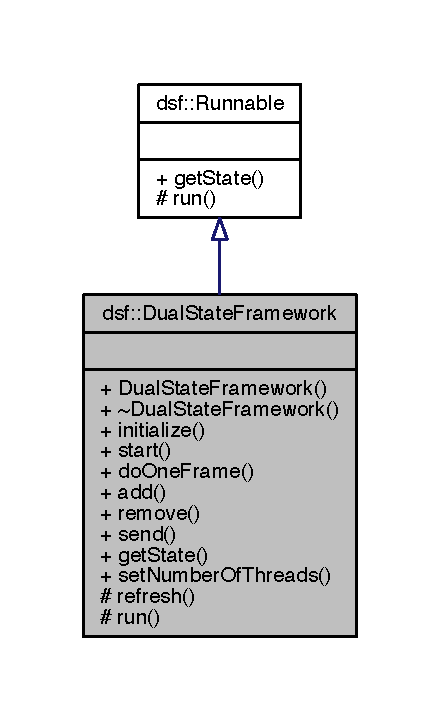
\includegraphics[width=211pt]{classdsf_1_1_dual_state_framework__inherit__graph}
\end{center}
\end{figure}
\subsection*{Public Member Functions}
\begin{DoxyCompactItemize}
\item 
\hyperlink{classdsf_1_1_dual_state_framework_ab2c3f064dee1876d92694544d032b942}{Dual\+State\+Framework} ()
\item 
\hyperlink{classdsf_1_1_dual_state_framework_a0e5246056c73a684d0a167f3ed6d1fb1}{$\sim$\+Dual\+State\+Framework} ()
\item 
virtual void \hyperlink{classdsf_1_1_dual_state_framework_a809a7bba4148e17ea9a43a0a035383ba}{initialize} ()=0
\item 
void \hyperlink{classdsf_1_1_dual_state_framework_ab17692c652ab856818d5e8f0dd82f194}{start} ()
\item 
void \hyperlink{classdsf_1_1_dual_state_framework_a72f0e6753a30394c0e505bb0bc481e3f}{do\+One\+Frame} ()
\item 
void \hyperlink{classdsf_1_1_dual_state_framework_a2ce40c8e165a8ed8fd6cb6cb30ae985b}{add} (\hyperlink{classdsf_1_1_synchronized_object}{Synchronized\+Object} $\ast$sync\+Obj)
\item 
void \hyperlink{classdsf_1_1_dual_state_framework_ab6ca84c5186f4fc3e048c4ff7a104ae7}{remove} (\hyperlink{classdsf_1_1_synchronized_object}{Synchronized\+Object} $\ast$sync\+Obj)
\item 
void \hyperlink{classdsf_1_1_dual_state_framework_a3063d7f0ce537eb44dc2bdcec816a36b}{send} (\hyperlink{classdsf_1_1_synchronized_object}{Synchronized\+Object} $\ast$to, \hyperlink{classdsf_1_1_synchronized_object}{Synchronized\+Object} $\ast$from, \hyperlink{namespacedsf_aa16e735f29587f4485b56fc46746f7a9}{Task\+Function} $\ast$task\+Function, \hyperlink{namespacedsf_abe4bf68433935a81c31a5ada9b17663a}{Task\+Argument} $\ast$args)
\item 
\hyperlink{classdsf_1_1_runnable_a8eb63b21a0accc7a6a2a05f18e257991}{State} \hyperlink{classdsf_1_1_dual_state_framework_a9f41adffe986e0d9360e0bbfba2a245a}{get\+State} () override
\item 
void \hyperlink{classdsf_1_1_dual_state_framework_a8ab358a7456eeed264d53304b6562be4}{set\+Number\+Of\+Threads} (int Number\+Of\+Threads)
\end{DoxyCompactItemize}
\subsection*{Protected Member Functions}
\begin{DoxyCompactItemize}
\item 
virtual void \hyperlink{classdsf_1_1_dual_state_framework_ab4c6856bd4036f8abbc2be2c0f00ea1a}{refresh} ()
\item 
virtual void \hyperlink{classdsf_1_1_dual_state_framework_a7b40bcf755127022f9258e846ddedb23}{run} () override
\end{DoxyCompactItemize}
\subsection*{Additional Inherited Members}


\subsection{Detailed Description}
The starting pointer for the framework is the abstract class \hyperlink{classdsf_1_1_dual_state_framework}{dsf\+::\+Dual\+State\+Framework}. 

It provides essential functions for associating and managing its components (\hyperlink{classdsf_1_1_synchronized_object}{Synchronized\+Object} objects, function points, and etc.). \hypertarget{classdsf_1_1_synchronized_object_eg}{}\subsection{Example}\label{classdsf_1_1_synchronized_object_eg}

\begin{DoxyCodeInclude}
\textcolor{preprocessor}{#ifndef \_\_DSFExample\_\_MyDSF\_\_}
\textcolor{preprocessor}{#define \_\_DSFExample\_\_MyDSF\_\_}

\textcolor{preprocessor}{#include <dsf/DualStateFramework.h>}

\textcolor{keyword}{class }MyDSF : \textcolor{keyword}{public} \hyperlink{classdsf_1_1_dual_state_framework}{dsf::DualStateFramework} \textcolor{comment}{// Extends dsf::DualStateFramework}
\{
\textcolor{keyword}{public}:
    \textcolor{keyword}{explicit} MyDSF() : \hyperlink{classdsf_1_1_dual_state_framework_ab2c3f064dee1876d92694544d032b942}{DualStateFramework}() \{\} \textcolor{comment}{// Uses default super constructor}
    \textcolor{keywordtype}{void} \hyperlink{classdsf_1_1_dual_state_framework_a809a7bba4148e17ea9a43a0a035383ba}{initialize}()\textcolor{keyword}{ override }\{\}
\};

\textcolor{preprocessor}{#endif}
\end{DoxyCodeInclude}
 

\subsection{Constructor \& Destructor Documentation}
\hypertarget{classdsf_1_1_dual_state_framework_ab2c3f064dee1876d92694544d032b942}{}\index{dsf\+::\+Dual\+State\+Framework@{dsf\+::\+Dual\+State\+Framework}!Dual\+State\+Framework@{Dual\+State\+Framework}}
\index{Dual\+State\+Framework@{Dual\+State\+Framework}!dsf\+::\+Dual\+State\+Framework@{dsf\+::\+Dual\+State\+Framework}}
\subsubsection[{Dual\+State\+Framework}]{\setlength{\rightskip}{0pt plus 5cm}dsf\+::\+Dual\+State\+Framework\+::\+Dual\+State\+Framework (
\begin{DoxyParamCaption}
{}
\end{DoxyParamCaption}
)}\label{classdsf_1_1_dual_state_framework_ab2c3f064dee1876d92694544d032b942}
\hypertarget{classdsf_1_1_dual_state_framework_a0e5246056c73a684d0a167f3ed6d1fb1}{}\index{dsf\+::\+Dual\+State\+Framework@{dsf\+::\+Dual\+State\+Framework}!````~Dual\+State\+Framework@{$\sim$\+Dual\+State\+Framework}}
\index{````~Dual\+State\+Framework@{$\sim$\+Dual\+State\+Framework}!dsf\+::\+Dual\+State\+Framework@{dsf\+::\+Dual\+State\+Framework}}
\subsubsection[{$\sim$\+Dual\+State\+Framework}]{\setlength{\rightskip}{0pt plus 5cm}dsf\+::\+Dual\+State\+Framework\+::$\sim$\+Dual\+State\+Framework (
\begin{DoxyParamCaption}
{}
\end{DoxyParamCaption}
)}\label{classdsf_1_1_dual_state_framework_a0e5246056c73a684d0a167f3ed6d1fb1}


\subsection{Member Function Documentation}
\hypertarget{classdsf_1_1_dual_state_framework_a2ce40c8e165a8ed8fd6cb6cb30ae985b}{}\index{dsf\+::\+Dual\+State\+Framework@{dsf\+::\+Dual\+State\+Framework}!add@{add}}
\index{add@{add}!dsf\+::\+Dual\+State\+Framework@{dsf\+::\+Dual\+State\+Framework}}
\subsubsection[{add}]{\setlength{\rightskip}{0pt plus 5cm}void dsf\+::\+Dual\+State\+Framework\+::add (
\begin{DoxyParamCaption}
\item[{{\bf Synchronized\+Object} $\ast$}]{sync\+Obj}
\end{DoxyParamCaption}
)}\label{classdsf_1_1_dual_state_framework_a2ce40c8e165a8ed8fd6cb6cb30ae985b}
Add a \hyperlink{classdsf_1_1_synchronized_object}{Synchronized\+Object}. \hypertarget{classdsf_1_1_dual_state_framework_a72f0e6753a30394c0e505bb0bc481e3f}{}\index{dsf\+::\+Dual\+State\+Framework@{dsf\+::\+Dual\+State\+Framework}!do\+One\+Frame@{do\+One\+Frame}}
\index{do\+One\+Frame@{do\+One\+Frame}!dsf\+::\+Dual\+State\+Framework@{dsf\+::\+Dual\+State\+Framework}}
\subsubsection[{do\+One\+Frame}]{\setlength{\rightskip}{0pt plus 5cm}void dsf\+::\+Dual\+State\+Framework\+::do\+One\+Frame (
\begin{DoxyParamCaption}
{}
\end{DoxyParamCaption}
)}\label{classdsf_1_1_dual_state_framework_a72f0e6753a30394c0e505bb0bc481e3f}
Do one frame of all Syncronized\+Objects. \hypertarget{classdsf_1_1_dual_state_framework_a9f41adffe986e0d9360e0bbfba2a245a}{}\index{dsf\+::\+Dual\+State\+Framework@{dsf\+::\+Dual\+State\+Framework}!get\+State@{get\+State}}
\index{get\+State@{get\+State}!dsf\+::\+Dual\+State\+Framework@{dsf\+::\+Dual\+State\+Framework}}
\subsubsection[{get\+State}]{\setlength{\rightskip}{0pt plus 5cm}{\bf State} dsf\+::\+Dual\+State\+Framework\+::get\+State (
\begin{DoxyParamCaption}
{}
\end{DoxyParamCaption}
)\hspace{0.3cm}{\ttfamily [override]}, {\ttfamily [virtual]}}\label{classdsf_1_1_dual_state_framework_a9f41adffe986e0d9360e0bbfba2a245a}
Return the state of the object. 

Implements \hyperlink{classdsf_1_1_runnable_a139342b0d6d53fc7f1bbd97d99d3724a}{dsf\+::\+Runnable}.

\hypertarget{classdsf_1_1_dual_state_framework_a809a7bba4148e17ea9a43a0a035383ba}{}\index{dsf\+::\+Dual\+State\+Framework@{dsf\+::\+Dual\+State\+Framework}!initialize@{initialize}}
\index{initialize@{initialize}!dsf\+::\+Dual\+State\+Framework@{dsf\+::\+Dual\+State\+Framework}}
\subsubsection[{initialize}]{\setlength{\rightskip}{0pt plus 5cm}virtual void dsf\+::\+Dual\+State\+Framework\+::initialize (
\begin{DoxyParamCaption}
{}
\end{DoxyParamCaption}
)\hspace{0.3cm}{\ttfamily [pure virtual]}}\label{classdsf_1_1_dual_state_framework_a809a7bba4148e17ea9a43a0a035383ba}
For Signing Task\+Function Pointers\hypertarget{classdsf_1_1_synchronized_object_eg}{}\subsection{Example}\label{classdsf_1_1_synchronized_object_eg}

\begin{DoxyCode}
this->printHello = \textcolor{keyword}{new} \hyperlink{namespacedsf_aa16e735f29587f4485b56fc46746f7a9}{dsf::TaskFunction}([\textcolor{keyword}{this}](
      \hyperlink{classdsf_1_1_synchronized_object}{dsf::SynchronizedObject}* to,
                                                \hyperlink{classdsf_1_1_synchronized_object}{dsf::SynchronizedObject}* from,
                                                \hyperlink{namespacedsf_abe4bf68433935a81c31a5ada9b17663a}{dsf::TaskArgument}* args)
\{
   std::string str;
   \textcolor{keywordtype}{float} f;
   std::tie(str, f) = args->to<std::tuple<std::string, float>>();
   std::cout << str << \textcolor{stringliteral}{" "} << f << std::endl;
   this->\textcolor{keyword}{remove}(from);
\});
\end{DoxyCode}
 \hypertarget{classdsf_1_1_dual_state_framework_ab4c6856bd4036f8abbc2be2c0f00ea1a}{}\index{dsf\+::\+Dual\+State\+Framework@{dsf\+::\+Dual\+State\+Framework}!refresh@{refresh}}
\index{refresh@{refresh}!dsf\+::\+Dual\+State\+Framework@{dsf\+::\+Dual\+State\+Framework}}
\subsubsection[{refresh}]{\setlength{\rightskip}{0pt plus 5cm}virtual void dsf\+::\+Dual\+State\+Framework\+::refresh (
\begin{DoxyParamCaption}
{}
\end{DoxyParamCaption}
)\hspace{0.3cm}{\ttfamily [protected]}, {\ttfamily [virtual]}}\label{classdsf_1_1_dual_state_framework_ab4c6856bd4036f8abbc2be2c0f00ea1a}
Clear all Syncronized\+Objects which is marked as D\+E\+L\+E\+T\+E \hypertarget{classdsf_1_1_dual_state_framework_ab6ca84c5186f4fc3e048c4ff7a104ae7}{}\index{dsf\+::\+Dual\+State\+Framework@{dsf\+::\+Dual\+State\+Framework}!remove@{remove}}
\index{remove@{remove}!dsf\+::\+Dual\+State\+Framework@{dsf\+::\+Dual\+State\+Framework}}
\subsubsection[{remove}]{\setlength{\rightskip}{0pt plus 5cm}void dsf\+::\+Dual\+State\+Framework\+::remove (
\begin{DoxyParamCaption}
\item[{{\bf Synchronized\+Object} $\ast$}]{sync\+Obj}
\end{DoxyParamCaption}
)}\label{classdsf_1_1_dual_state_framework_ab6ca84c5186f4fc3e048c4ff7a104ae7}
Remove a \hyperlink{classdsf_1_1_synchronized_object}{Synchronized\+Object}. \hypertarget{classdsf_1_1_dual_state_framework_a7b40bcf755127022f9258e846ddedb23}{}\index{dsf\+::\+Dual\+State\+Framework@{dsf\+::\+Dual\+State\+Framework}!run@{run}}
\index{run@{run}!dsf\+::\+Dual\+State\+Framework@{dsf\+::\+Dual\+State\+Framework}}
\subsubsection[{run}]{\setlength{\rightskip}{0pt plus 5cm}virtual void dsf\+::\+Dual\+State\+Framework\+::run (
\begin{DoxyParamCaption}
{}
\end{DoxyParamCaption}
)\hspace{0.3cm}{\ttfamily [override]}, {\ttfamily [protected]}, {\ttfamily [virtual]}}\label{classdsf_1_1_dual_state_framework_a7b40bcf755127022f9258e846ddedb23}
Start all Syncronized\+Objects associated. 

Implements \hyperlink{classdsf_1_1_runnable_a6e23b3b551a7cfdbff0e9ba2265d4378}{dsf\+::\+Runnable}.

\hypertarget{classdsf_1_1_dual_state_framework_a3063d7f0ce537eb44dc2bdcec816a36b}{}\index{dsf\+::\+Dual\+State\+Framework@{dsf\+::\+Dual\+State\+Framework}!send@{send}}
\index{send@{send}!dsf\+::\+Dual\+State\+Framework@{dsf\+::\+Dual\+State\+Framework}}
\subsubsection[{send}]{\setlength{\rightskip}{0pt plus 5cm}void dsf\+::\+Dual\+State\+Framework\+::send (
\begin{DoxyParamCaption}
\item[{{\bf Synchronized\+Object} $\ast$}]{to, }
\item[{{\bf Synchronized\+Object} $\ast$}]{from, }
\item[{{\bf Task\+Function} $\ast$}]{task\+Function, }
\item[{{\bf Task\+Argument} $\ast$}]{args}
\end{DoxyParamCaption}
)}\label{classdsf_1_1_dual_state_framework_a3063d7f0ce537eb44dc2bdcec816a36b}
Send messages \hypertarget{classdsf_1_1_dual_state_framework_a8ab358a7456eeed264d53304b6562be4}{}\index{dsf\+::\+Dual\+State\+Framework@{dsf\+::\+Dual\+State\+Framework}!set\+Number\+Of\+Threads@{set\+Number\+Of\+Threads}}
\index{set\+Number\+Of\+Threads@{set\+Number\+Of\+Threads}!dsf\+::\+Dual\+State\+Framework@{dsf\+::\+Dual\+State\+Framework}}
\subsubsection[{set\+Number\+Of\+Threads}]{\setlength{\rightskip}{0pt plus 5cm}void dsf\+::\+Dual\+State\+Framework\+::set\+Number\+Of\+Threads (
\begin{DoxyParamCaption}
\item[{int}]{Number\+Of\+Threads}
\end{DoxyParamCaption}
)}\label{classdsf_1_1_dual_state_framework_a8ab358a7456eeed264d53304b6562be4}
Set the number of threads. 0 is automatic. \hypertarget{classdsf_1_1_dual_state_framework_ab17692c652ab856818d5e8f0dd82f194}{}\index{dsf\+::\+Dual\+State\+Framework@{dsf\+::\+Dual\+State\+Framework}!start@{start}}
\index{start@{start}!dsf\+::\+Dual\+State\+Framework@{dsf\+::\+Dual\+State\+Framework}}
\subsubsection[{start}]{\setlength{\rightskip}{0pt plus 5cm}void dsf\+::\+Dual\+State\+Framework\+::start (
\begin{DoxyParamCaption}
{}
\end{DoxyParamCaption}
)}\label{classdsf_1_1_dual_state_framework_ab17692c652ab856818d5e8f0dd82f194}
Start all Syncronized\+Objects associated. 

The documentation for this class was generated from the following file\+:\begin{DoxyCompactItemize}
\item 
Dual\+State\+Framework.\+h\end{DoxyCompactItemize}

\hypertarget{classdsf_1_1_lock}{}\section{dsf\+:\+:Lock Class Reference}
\label{classdsf_1_1_lock}\index{dsf\+::\+Lock@{dsf\+::\+Lock}}


Locking variables.  




{\ttfamily \#include $<$Lock.\+h$>$}



Inheritance diagram for dsf\+:\+:Lock\+:\nopagebreak
\begin{figure}[H]
\begin{center}
\leavevmode
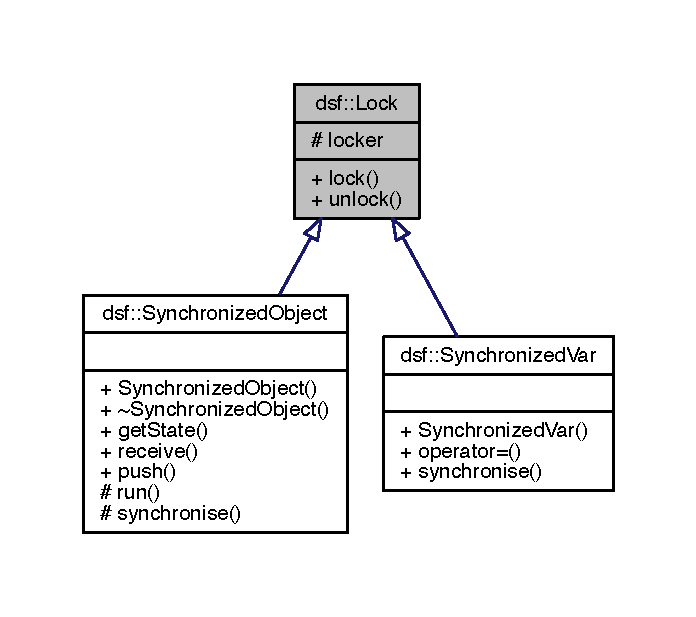
\includegraphics[width=334pt]{classdsf_1_1_lock__inherit__graph}
\end{center}
\end{figure}
\subsection*{Public Member Functions}
\begin{DoxyCompactItemize}
\item 
void \hyperlink{classdsf_1_1_lock_ae521388d861fe66b9c6e2f09811b0d4b}{lock} ()
\item 
void \hyperlink{classdsf_1_1_lock_a3d03f801920d458b3c3c402a0f4af323}{unlock} ()
\end{DoxyCompactItemize}
\subsection*{Protected Attributes}
\begin{DoxyCompactItemize}
\item 
std\+::mutex \hyperlink{classdsf_1_1_lock_a605f27e33e37dc8b3b920a3272461c44}{locker}
\end{DoxyCompactItemize}


\subsection{Detailed Description}
Locking variables. 

The class can lock the objects using an unspecified sequence of calls to their members lock and unlock that ensures that all arguments are locked on return (without producing any deadlocks).\hypertarget{classdsf_1_1_synchronized_object_eg}{}\subsection{Example}\label{classdsf_1_1_synchronized_object_eg}

\begin{DoxyCode}
\hyperlink{namespacedsf}{dsf}->lock();
\hyperlink{namespacedsf}{dsf}->drawables->push\_back(syncObj); \textcolor{comment}{//the object drawables is locked}
\hyperlink{namespacedsf}{dsf}->unlock();
\end{DoxyCode}
 

\subsection{Member Function Documentation}
\hypertarget{classdsf_1_1_lock_ae521388d861fe66b9c6e2f09811b0d4b}{}\index{dsf\+::\+Lock@{dsf\+::\+Lock}!lock@{lock}}
\index{lock@{lock}!dsf\+::\+Lock@{dsf\+::\+Lock}}
\subsubsection[{lock}]{\setlength{\rightskip}{0pt plus 5cm}void dsf\+::\+Lock\+::lock (
\begin{DoxyParamCaption}
{}
\end{DoxyParamCaption}
)}\label{classdsf_1_1_lock_ae521388d861fe66b9c6e2f09811b0d4b}
Locks all the objects passed as arguments, blocking the calling thread if necessary. 

Here is the caller graph for this function\+:\nopagebreak
\begin{figure}[H]
\begin{center}
\leavevmode
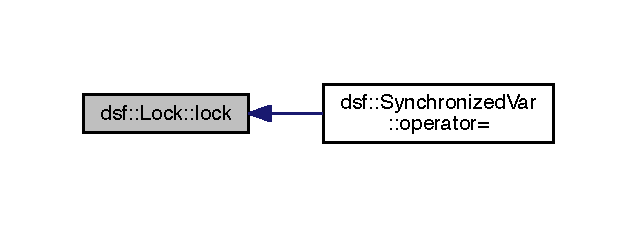
\includegraphics[width=306pt]{classdsf_1_1_lock_ae521388d861fe66b9c6e2f09811b0d4b_icgraph}
\end{center}
\end{figure}


\hypertarget{classdsf_1_1_lock_a3d03f801920d458b3c3c402a0f4af323}{}\index{dsf\+::\+Lock@{dsf\+::\+Lock}!unlock@{unlock}}
\index{unlock@{unlock}!dsf\+::\+Lock@{dsf\+::\+Lock}}
\subsubsection[{unlock}]{\setlength{\rightskip}{0pt plus 5cm}void dsf\+::\+Lock\+::unlock (
\begin{DoxyParamCaption}
{}
\end{DoxyParamCaption}
)}\label{classdsf_1_1_lock_a3d03f801920d458b3c3c402a0f4af323}
Unlocks all the objects. 

Here is the caller graph for this function\+:\nopagebreak
\begin{figure}[H]
\begin{center}
\leavevmode
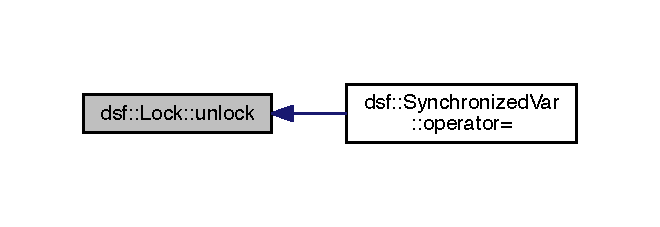
\includegraphics[width=317pt]{classdsf_1_1_lock_a3d03f801920d458b3c3c402a0f4af323_icgraph}
\end{center}
\end{figure}




\subsection{Member Data Documentation}
\hypertarget{classdsf_1_1_lock_a605f27e33e37dc8b3b920a3272461c44}{}\index{dsf\+::\+Lock@{dsf\+::\+Lock}!locker@{locker}}
\index{locker@{locker}!dsf\+::\+Lock@{dsf\+::\+Lock}}
\subsubsection[{locker}]{\setlength{\rightskip}{0pt plus 5cm}std\+::mutex dsf\+::\+Lock\+::locker\hspace{0.3cm}{\ttfamily [protected]}}\label{classdsf_1_1_lock_a605f27e33e37dc8b3b920a3272461c44}
The locker 

The documentation for this class was generated from the following file\+:\begin{DoxyCompactItemize}
\item 
Lock.\+h\end{DoxyCompactItemize}

\hypertarget{classdsf_1_1_runnable}{}\section{dsf\+:\+:Runnable Class Reference}
\label{classdsf_1_1_runnable}\index{dsf\+::\+Runnable@{dsf\+::\+Runnable}}


Executing messages.  




{\ttfamily \#include $<$Runnable.\+h$>$}



Inheritance diagram for dsf\+:\+:Runnable\+:\nopagebreak
\begin{figure}[H]
\begin{center}
\leavevmode
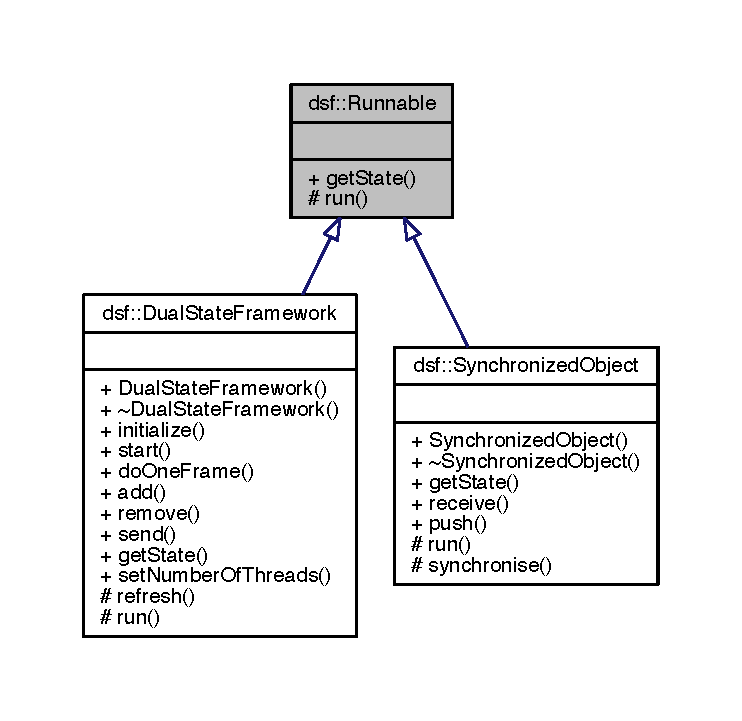
\includegraphics[width=350pt]{classdsf_1_1_runnable__inherit__graph}
\end{center}
\end{figure}
\subsection*{Public Types}
\begin{DoxyCompactItemize}
\item 
enum \hyperlink{classdsf_1_1_runnable_a8eb63b21a0accc7a6a2a05f18e257991}{State} \{ \hyperlink{classdsf_1_1_runnable_a8eb63b21a0accc7a6a2a05f18e257991ad7167727fe5c31678c166aee6801ba0a}{R\+U\+N\+N\+I\+N\+G}, 
\hyperlink{classdsf_1_1_runnable_a8eb63b21a0accc7a6a2a05f18e257991a0897925165e6577c4d3ebb185178c9c5}{S\+T\+O\+P\+P\+E\+D}, 
\hyperlink{classdsf_1_1_runnable_a8eb63b21a0accc7a6a2a05f18e257991a60038f4f186bbe0d05fdbbe9da0f85de}{R\+E\+A\+D\+Y}, 
\hyperlink{classdsf_1_1_runnable_a8eb63b21a0accc7a6a2a05f18e257991aea5cfe327f95ca42d589e660b7cffe28}{D\+E\+L\+E\+T\+E\+D}
 \}
\begin{DoxyCompactList}\small\item\em State of the object. \end{DoxyCompactList}\end{DoxyCompactItemize}
\subsection*{Public Member Functions}
\begin{DoxyCompactItemize}
\item 
virtual \hyperlink{classdsf_1_1_runnable_a8eb63b21a0accc7a6a2a05f18e257991}{State} \hyperlink{classdsf_1_1_runnable_a139342b0d6d53fc7f1bbd97d99d3724a}{get\+State} ()=0
\end{DoxyCompactItemize}
\subsection*{Protected Member Functions}
\begin{DoxyCompactItemize}
\item 
virtual void \hyperlink{classdsf_1_1_runnable_a6e23b3b551a7cfdbff0e9ba2265d4378}{run} ()=0
\end{DoxyCompactItemize}


\subsection{Detailed Description}
Executing messages. 

The interface provides a run method which executes messages. 

\subsection{Member Enumeration Documentation}
\hypertarget{classdsf_1_1_runnable_a8eb63b21a0accc7a6a2a05f18e257991}{}\index{dsf\+::\+Runnable@{dsf\+::\+Runnable}!State@{State}}
\index{State@{State}!dsf\+::\+Runnable@{dsf\+::\+Runnable}}
\subsubsection[{State}]{\setlength{\rightskip}{0pt plus 5cm}enum {\bf dsf\+::\+Runnable\+::\+State}}\label{classdsf_1_1_runnable_a8eb63b21a0accc7a6a2a05f18e257991}


State of the object. 

R\+U\+N\+N\+I\+N\+G\+: The object is running. ~\newline
 S\+T\+O\+P\+P\+E\+D\+: The object is stopped. ~\newline
 R\+E\+A\+D\+Y\+: The object is ready to run. ~\newline
 D\+E\+L\+E\+T\+E\+D\+: The object is marked as deleted. System will automatically delete it. \begin{Desc}
\item[Enumerator]\par
\begin{description}
\index{R\+U\+N\+N\+I\+N\+G@{R\+U\+N\+N\+I\+N\+G}!dsf\+::\+Runnable@{dsf\+::\+Runnable}}\index{dsf\+::\+Runnable@{dsf\+::\+Runnable}!R\+U\+N\+N\+I\+N\+G@{R\+U\+N\+N\+I\+N\+G}}\item[{\em 
\hypertarget{classdsf_1_1_runnable_a8eb63b21a0accc7a6a2a05f18e257991ad7167727fe5c31678c166aee6801ba0a}{}R\+U\+N\+N\+I\+N\+G\label{classdsf_1_1_runnable_a8eb63b21a0accc7a6a2a05f18e257991ad7167727fe5c31678c166aee6801ba0a}
}]\index{S\+T\+O\+P\+P\+E\+D@{S\+T\+O\+P\+P\+E\+D}!dsf\+::\+Runnable@{dsf\+::\+Runnable}}\index{dsf\+::\+Runnable@{dsf\+::\+Runnable}!S\+T\+O\+P\+P\+E\+D@{S\+T\+O\+P\+P\+E\+D}}\item[{\em 
\hypertarget{classdsf_1_1_runnable_a8eb63b21a0accc7a6a2a05f18e257991a0897925165e6577c4d3ebb185178c9c5}{}S\+T\+O\+P\+P\+E\+D\label{classdsf_1_1_runnable_a8eb63b21a0accc7a6a2a05f18e257991a0897925165e6577c4d3ebb185178c9c5}
}]\index{R\+E\+A\+D\+Y@{R\+E\+A\+D\+Y}!dsf\+::\+Runnable@{dsf\+::\+Runnable}}\index{dsf\+::\+Runnable@{dsf\+::\+Runnable}!R\+E\+A\+D\+Y@{R\+E\+A\+D\+Y}}\item[{\em 
\hypertarget{classdsf_1_1_runnable_a8eb63b21a0accc7a6a2a05f18e257991a60038f4f186bbe0d05fdbbe9da0f85de}{}R\+E\+A\+D\+Y\label{classdsf_1_1_runnable_a8eb63b21a0accc7a6a2a05f18e257991a60038f4f186bbe0d05fdbbe9da0f85de}
}]\index{D\+E\+L\+E\+T\+E\+D@{D\+E\+L\+E\+T\+E\+D}!dsf\+::\+Runnable@{dsf\+::\+Runnable}}\index{dsf\+::\+Runnable@{dsf\+::\+Runnable}!D\+E\+L\+E\+T\+E\+D@{D\+E\+L\+E\+T\+E\+D}}\item[{\em 
\hypertarget{classdsf_1_1_runnable_a8eb63b21a0accc7a6a2a05f18e257991aea5cfe327f95ca42d589e660b7cffe28}{}D\+E\+L\+E\+T\+E\+D\label{classdsf_1_1_runnable_a8eb63b21a0accc7a6a2a05f18e257991aea5cfe327f95ca42d589e660b7cffe28}
}]\end{description}
\end{Desc}


\subsection{Member Function Documentation}
\hypertarget{classdsf_1_1_runnable_a139342b0d6d53fc7f1bbd97d99d3724a}{}\index{dsf\+::\+Runnable@{dsf\+::\+Runnable}!get\+State@{get\+State}}
\index{get\+State@{get\+State}!dsf\+::\+Runnable@{dsf\+::\+Runnable}}
\subsubsection[{get\+State}]{\setlength{\rightskip}{0pt plus 5cm}virtual {\bf State} dsf\+::\+Runnable\+::get\+State (
\begin{DoxyParamCaption}
{}
\end{DoxyParamCaption}
)\hspace{0.3cm}{\ttfamily [pure virtual]}}\label{classdsf_1_1_runnable_a139342b0d6d53fc7f1bbd97d99d3724a}
Returns the current state. 

Implemented in \hyperlink{classdsf_1_1_dual_state_framework_a9f41adffe986e0d9360e0bbfba2a245a}{dsf\+::\+Dual\+State\+Framework}, and \hyperlink{classdsf_1_1_synchronized_object_a744c49c3f58728492b97a167e2d83d02}{dsf\+::\+Synchronized\+Object}.

\hypertarget{classdsf_1_1_runnable_a6e23b3b551a7cfdbff0e9ba2265d4378}{}\index{dsf\+::\+Runnable@{dsf\+::\+Runnable}!run@{run}}
\index{run@{run}!dsf\+::\+Runnable@{dsf\+::\+Runnable}}
\subsubsection[{run}]{\setlength{\rightskip}{0pt plus 5cm}virtual void dsf\+::\+Runnable\+::run (
\begin{DoxyParamCaption}
{}
\end{DoxyParamCaption}
)\hspace{0.3cm}{\ttfamily [protected]}, {\ttfamily [pure virtual]}}\label{classdsf_1_1_runnable_a6e23b3b551a7cfdbff0e9ba2265d4378}
Executes messages 

Implemented in \hyperlink{classdsf_1_1_dual_state_framework_a7b40bcf755127022f9258e846ddedb23}{dsf\+::\+Dual\+State\+Framework}, and \hyperlink{classdsf_1_1_synchronized_object_ae94875bd63d8071f8a563ac45ca7ccc2}{dsf\+::\+Synchronized\+Object}.



The documentation for this class was generated from the following file\+:\begin{DoxyCompactItemize}
\item 
/\+Users/yuchen/\+Repositories/\+Dual\+State\+Framework/dsf/include/dsf/Runnable.\+h\end{DoxyCompactItemize}

\hypertarget{classdsf_1_1_synchronisable}{}\section{dsf\+:\+:Synchronisable$<$ T $>$ Class Template Reference}
\label{classdsf_1_1_synchronisable}\index{dsf\+::\+Synchronisable$<$ T $>$@{dsf\+::\+Synchronisable$<$ T $>$}}


Synchronising two states.  




{\ttfamily \#include $<$Synchronisable.\+h$>$}

\subsection*{Public Member Functions}
\begin{DoxyCompactItemize}
\item 
virtual \hyperlink{classdsf_1_1_synchronisable_ae733344b5ac5742826aa4781abdc6e2c}{$\sim$\+Synchronisable} ()
\item 
virtual void \hyperlink{classdsf_1_1_synchronisable_a225f9a5f6cb47d73e1ea4d788bbfcaaa}{synchronise} ()=0
\end{DoxyCompactItemize}
\subsection*{Protected Attributes}
\begin{DoxyCompactItemize}
\item 
T $\ast$ \hyperlink{classdsf_1_1_synchronisable_ae2434faac15d3184da1543a91e175713}{next}
\end{DoxyCompactItemize}


\subsection{Detailed Description}
\subsubsection*{template$<$class T$>$class dsf\+::\+Synchronisable$<$ T $>$}

Synchronising two states. 

The template interface provides a copy of current object, and a synchronise method which synchronise two copies. \hypertarget{classdsf_1_1_synchronized_var_Example}{}\subsection{Example}\label{classdsf_1_1_synchronized_var_Example}

\begin{DoxyCode}
\textcolor{preprocessor}{#include <\hyperlink{_synchronisable_8h}{dsf/Synchronisable.h}>}

\textcolor{keyword}{class }Vector3D
\{
\textcolor{keyword}{public}:
    \textcolor{keywordtype}{float} x, y, z;
    Vector3D(\textcolor{keywordtype}{float} x, \textcolor{keywordtype}{float} y, \textcolor{keywordtype}{float} z) : x(x), y(y), z(z)\{\}
\}

\textcolor{keyword}{class }SyncVector : \textcolor{keyword}{public} \hyperlink{classdsf_1_1_synchronisable}{dsf::Synchronisable}<Vector3D>, \textcolor{keyword}{public} Vector3D
\{
\textcolor{keyword}{public}:
    SyncInt(\textcolor{keywordtype}{float} x, \textcolor{keywordtype}{float} y, \textcolor{keywordtype}{float} z) : Vector3D(x, y, z) \{
        this->\hyperlink{classdsf_1_1_synchronisable_ae2434faac15d3184da1543a91e175713}{next} = \textcolor{keyword}{new} Vector3D(x, y, z);
    \}
    \textcolor{keywordtype}{void} \hyperlink{classdsf_1_1_synchronisable_a225f9a5f6cb47d73e1ea4d788bbfcaaa}{synchronise}()\textcolor{keyword}{ override }\{
        this->x = this->\hyperlink{classdsf_1_1_synchronisable_ae2434faac15d3184da1543a91e175713}{next}->x;
        this->y = this->\hyperlink{classdsf_1_1_synchronisable_ae2434faac15d3184da1543a91e175713}{next}->y;
        this->z = this->\hyperlink{classdsf_1_1_synchronisable_ae2434faac15d3184da1543a91e175713}{next}->z;
    \}
\}
\end{DoxyCode}
 

\subsection{Constructor \& Destructor Documentation}
\hypertarget{classdsf_1_1_synchronisable_ae733344b5ac5742826aa4781abdc6e2c}{}\index{dsf\+::\+Synchronisable@{dsf\+::\+Synchronisable}!````~Synchronisable@{$\sim$\+Synchronisable}}
\index{````~Synchronisable@{$\sim$\+Synchronisable}!dsf\+::\+Synchronisable@{dsf\+::\+Synchronisable}}
\subsubsection[{$\sim$\+Synchronisable}]{\setlength{\rightskip}{0pt plus 5cm}template$<$class T$>$ virtual {\bf dsf\+::\+Synchronisable}$<$ T $>$\+::$\sim${\bf Synchronisable} (
\begin{DoxyParamCaption}
{}
\end{DoxyParamCaption}
)\hspace{0.3cm}{\ttfamily [inline]}, {\ttfamily [virtual]}}\label{classdsf_1_1_synchronisable_ae733344b5ac5742826aa4781abdc6e2c}


\subsection{Member Function Documentation}
\hypertarget{classdsf_1_1_synchronisable_a225f9a5f6cb47d73e1ea4d788bbfcaaa}{}\index{dsf\+::\+Synchronisable@{dsf\+::\+Synchronisable}!synchronise@{synchronise}}
\index{synchronise@{synchronise}!dsf\+::\+Synchronisable@{dsf\+::\+Synchronisable}}
\subsubsection[{synchronise}]{\setlength{\rightskip}{0pt plus 5cm}template$<$class T$>$ virtual void {\bf dsf\+::\+Synchronisable}$<$ T $>$\+::synchronise (
\begin{DoxyParamCaption}
{}
\end{DoxyParamCaption}
)\hspace{0.3cm}{\ttfamily [pure virtual]}}\label{classdsf_1_1_synchronisable_a225f9a5f6cb47d73e1ea4d788bbfcaaa}
Signs current value to next value. 

Implemented in \hyperlink{classdsf_1_1_synchronized_object_a4e200d7b3508db98f09c6fe547f46cdb}{dsf\+::\+Synchronized\+Object}, and \hyperlink{classdsf_1_1_synchronized_var_ac8465a885c4dbb5bc5ca9ad25f42c3ec}{dsf\+::\+Synchronized\+Var}.



\subsection{Member Data Documentation}
\hypertarget{classdsf_1_1_synchronisable_ae2434faac15d3184da1543a91e175713}{}\index{dsf\+::\+Synchronisable@{dsf\+::\+Synchronisable}!next@{next}}
\index{next@{next}!dsf\+::\+Synchronisable@{dsf\+::\+Synchronisable}}
\subsubsection[{next}]{\setlength{\rightskip}{0pt plus 5cm}template$<$class T$>$ T$\ast$ {\bf dsf\+::\+Synchronisable}$<$ T $>$\+::next\hspace{0.3cm}{\ttfamily [protected]}}\label{classdsf_1_1_synchronisable_ae2434faac15d3184da1543a91e175713}
A copy of current object. 

The documentation for this class was generated from the following file\+:\begin{DoxyCompactItemize}
\item 
/\+Users/yuchen/\+Repositories/\+Dual\+State\+Framework/dsf/include/dsf/\hyperlink{_synchronisable_8h}{Synchronisable.\+h}\end{DoxyCompactItemize}

\hypertarget{classdsf_1_1_synchronized_object}{}\section{dsf\+:\+:Synchronized\+Object Class Reference}
\label{classdsf_1_1_synchronized_object}\index{dsf\+::\+Synchronized\+Object@{dsf\+::\+Synchronized\+Object}}


Dual state object interface.  




{\ttfamily \#include $<$Synchronized\+Object.\+h$>$}



Inheritance diagram for dsf\+:\+:Synchronized\+Object\+:\nopagebreak
\begin{figure}[H]
\begin{center}
\leavevmode
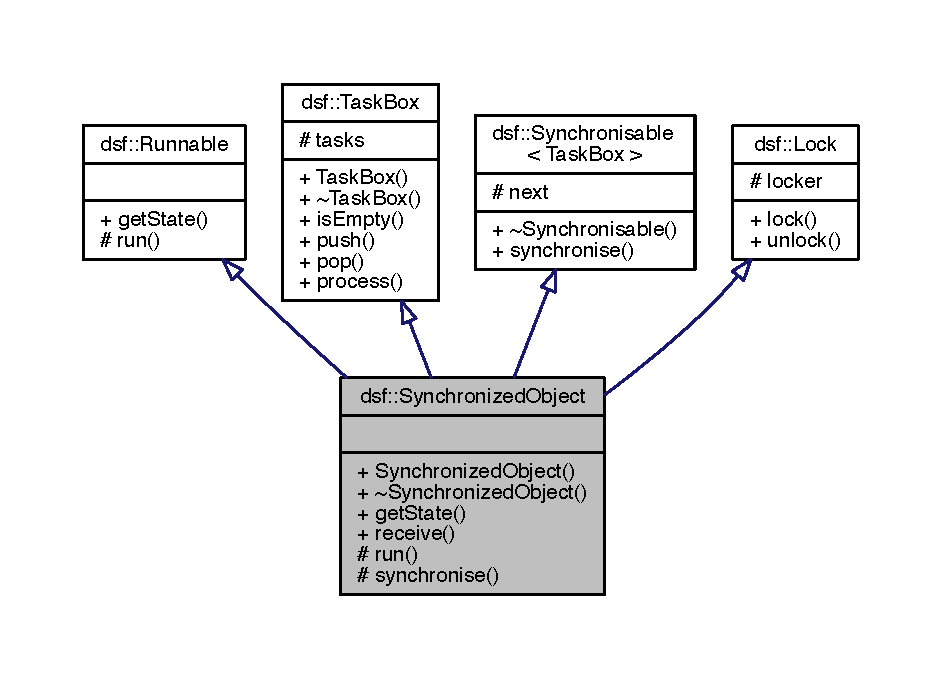
\includegraphics[width=350pt]{classdsf_1_1_synchronized_object__inherit__graph}
\end{center}
\end{figure}
\subsection*{Public Member Functions}
\begin{DoxyCompactItemize}
\item 
\hyperlink{classdsf_1_1_synchronized_object_a3f1d2def677e6d814de4d0bd2aa3d95b}{Synchronized\+Object} ()
\item 
virtual \hyperlink{classdsf_1_1_synchronized_object_a0181452530628f24baad25eea03580f9}{$\sim$\+Synchronized\+Object} ()
\item 
\hyperlink{classdsf_1_1_runnable_a8eb63b21a0accc7a6a2a05f18e257991}{State} \hyperlink{classdsf_1_1_synchronized_object_a9fbf045eff345188935402ae576933eb}{get\+State} () override
\item 
int \hyperlink{classdsf_1_1_synchronized_object_a3ce496c6aaecc4b0ca3a4d09539a4920}{receive} ()
\end{DoxyCompactItemize}
\subsection*{Protected Member Functions}
\begin{DoxyCompactItemize}
\item 
virtual void \hyperlink{classdsf_1_1_synchronized_object_ae94875bd63d8071f8a563ac45ca7ccc2}{run} () override=0
\item 
void \hyperlink{classdsf_1_1_synchronized_object_a4e200d7b3508db98f09c6fe547f46cdb}{synchronise} () override
\end{DoxyCompactItemize}
\subsection*{Friends}
\begin{DoxyCompactItemize}
\item 
class \hyperlink{classdsf_1_1_synchronized_object_a86db03c65431cb461cc8abf33bd2e74a}{Dual\+State\+Framework}
\end{DoxyCompactItemize}
\subsection*{Additional Inherited Members}


\subsection{Detailed Description}
Dual state object interface. 

The \hyperlink{classdsf_1_1_synchronized_object}{dsf\+::\+Synchronized\+Object} is a subclass of \hyperlink{classdsf_1_1_task_box}{dsf\+::\+Task\+Box}. In this framework, you can regard it as thread. It provides methods for implementing parallelism such as “send”, “receive”, and etc.\hypertarget{classdsf_1_1_synchronized_var_Example}{}\subsection{Example}\label{classdsf_1_1_synchronized_var_Example}

\begin{DoxyCode}
\textcolor{comment}{// SyncCircle.h}

\textcolor{preprocessor}{#include <dsf/SynchronizedObject.h>}
\textcolor{preprocessor}{#include <SFML/Graphics.hpp>}

\textcolor{keyword}{class }SyncCircle : \textcolor{keyword}{public} \hyperlink{classdsf_1_1_synchronized_object}{dsf::SynchronizedObject}, \textcolor{keyword}{public} sf::CircleShape
\{
\textcolor{keyword}{public}:
   SyncCircle();
\textcolor{keyword}{protected}:
   \textcolor{keywordtype}{void} \hyperlink{classdsf_1_1_synchronized_object_ae94875bd63d8071f8a563ac45ca7ccc2}{run}() \textcolor{keyword}{override};
\};


\textcolor{comment}{// SyncCircle.cpp}

\textcolor{preprocessor}{#include "SyncCircle.h"}

SyncCircle::SyncCircle()  : \hyperlink{namespacedsf}{dsf}::\hyperlink{classdsf_1_1_synchronized_object_a3f1d2def677e6d814de4d0bd2aa3d95b}{SynchronizedObject}::
      \hyperlink{classdsf_1_1_synchronized_object_a3f1d2def677e6d814de4d0bd2aa3d95b}{SynchronizedObject}(), sf::CircleShape::CircleShape()
\{
\}

\textcolor{keywordtype}{void} SyncCircle::run()
\{
   \textcolor{keywordflow}{if}(this->receive())
       this->process();
\}
\end{DoxyCode}
 

\subsection{Constructor \& Destructor Documentation}
\hypertarget{classdsf_1_1_synchronized_object_a3f1d2def677e6d814de4d0bd2aa3d95b}{}\index{dsf\+::\+Synchronized\+Object@{dsf\+::\+Synchronized\+Object}!Synchronized\+Object@{Synchronized\+Object}}
\index{Synchronized\+Object@{Synchronized\+Object}!dsf\+::\+Synchronized\+Object@{dsf\+::\+Synchronized\+Object}}
\subsubsection[{Synchronized\+Object}]{\setlength{\rightskip}{0pt plus 5cm}dsf\+::\+Synchronized\+Object\+::\+Synchronized\+Object (
\begin{DoxyParamCaption}
{}
\end{DoxyParamCaption}
)}\label{classdsf_1_1_synchronized_object_a3f1d2def677e6d814de4d0bd2aa3d95b}


Here is the call graph for this function\+:\nopagebreak
\begin{figure}[H]
\begin{center}
\leavevmode
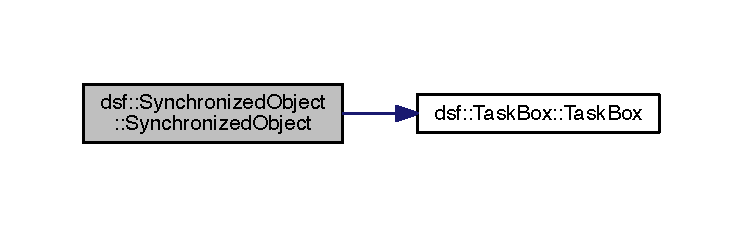
\includegraphics[width=350pt]{classdsf_1_1_synchronized_object_a3f1d2def677e6d814de4d0bd2aa3d95b_cgraph}
\end{center}
\end{figure}


\hypertarget{classdsf_1_1_synchronized_object_a0181452530628f24baad25eea03580f9}{}\index{dsf\+::\+Synchronized\+Object@{dsf\+::\+Synchronized\+Object}!````~Synchronized\+Object@{$\sim$\+Synchronized\+Object}}
\index{````~Synchronized\+Object@{$\sim$\+Synchronized\+Object}!dsf\+::\+Synchronized\+Object@{dsf\+::\+Synchronized\+Object}}
\subsubsection[{$\sim$\+Synchronized\+Object}]{\setlength{\rightskip}{0pt plus 5cm}dsf\+::\+Synchronized\+Object\+::$\sim$\+Synchronized\+Object (
\begin{DoxyParamCaption}
{}
\end{DoxyParamCaption}
)\hspace{0.3cm}{\ttfamily [virtual]}}\label{classdsf_1_1_synchronized_object_a0181452530628f24baad25eea03580f9}


\subsection{Member Function Documentation}
\hypertarget{classdsf_1_1_synchronized_object_a9fbf045eff345188935402ae576933eb}{}\index{dsf\+::\+Synchronized\+Object@{dsf\+::\+Synchronized\+Object}!get\+State@{get\+State}}
\index{get\+State@{get\+State}!dsf\+::\+Synchronized\+Object@{dsf\+::\+Synchronized\+Object}}
\subsubsection[{get\+State}]{\setlength{\rightskip}{0pt plus 5cm}{\bf Synchronized\+Object\+::\+State} dsf\+::\+Synchronized\+Object\+::get\+State (
\begin{DoxyParamCaption}
{}
\end{DoxyParamCaption}
)\hspace{0.3cm}{\ttfamily [override]}, {\ttfamily [virtual]}}\label{classdsf_1_1_synchronized_object_a9fbf045eff345188935402ae576933eb}
Returns the current state. 

Implements \hyperlink{classdsf_1_1_runnable_a139342b0d6d53fc7f1bbd97d99d3724a}{dsf\+::\+Runnable}.

\hypertarget{classdsf_1_1_synchronized_object_a3ce496c6aaecc4b0ca3a4d09539a4920}{}\index{dsf\+::\+Synchronized\+Object@{dsf\+::\+Synchronized\+Object}!receive@{receive}}
\index{receive@{receive}!dsf\+::\+Synchronized\+Object@{dsf\+::\+Synchronized\+Object}}
\subsubsection[{receive}]{\setlength{\rightskip}{0pt plus 5cm}int dsf\+::\+Synchronized\+Object\+::receive (
\begin{DoxyParamCaption}
{}
\end{DoxyParamCaption}
)}\label{classdsf_1_1_synchronized_object_a3ce496c6aaecc4b0ca3a4d09539a4920}
Returns the number of message received 

Here is the call graph for this function\+:\nopagebreak
\begin{figure}[H]
\begin{center}
\leavevmode
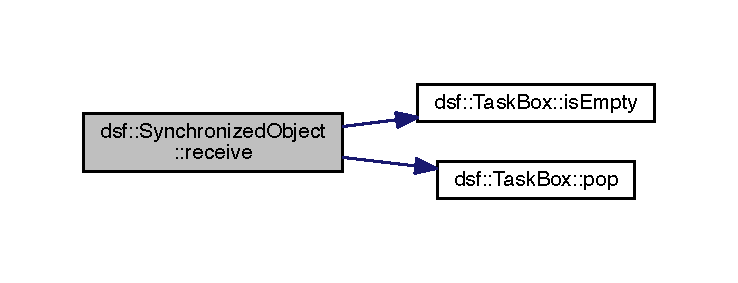
\includegraphics[width=350pt]{classdsf_1_1_synchronized_object_a3ce496c6aaecc4b0ca3a4d09539a4920_cgraph}
\end{center}
\end{figure}


\hypertarget{classdsf_1_1_synchronized_object_ae94875bd63d8071f8a563ac45ca7ccc2}{}\index{dsf\+::\+Synchronized\+Object@{dsf\+::\+Synchronized\+Object}!run@{run}}
\index{run@{run}!dsf\+::\+Synchronized\+Object@{dsf\+::\+Synchronized\+Object}}
\subsubsection[{run}]{\setlength{\rightskip}{0pt plus 5cm}virtual void dsf\+::\+Synchronized\+Object\+::run (
\begin{DoxyParamCaption}
{}
\end{DoxyParamCaption}
)\hspace{0.3cm}{\ttfamily [override]}, {\ttfamily [protected]}, {\ttfamily [pure virtual]}}\label{classdsf_1_1_synchronized_object_ae94875bd63d8071f8a563ac45ca7ccc2}
Executes messages \hypertarget{classdsf_1_1_synchronized_object_eg}{}\subsection{Example}\label{classdsf_1_1_synchronized_object_eg}

\begin{DoxyCode}
\textcolor{keywordtype}{void} \hyperlink{classdsf_1_1_synchronized_object_ae94875bd63d8071f8a563ac45ca7ccc2}{run}()\textcolor{keyword}{ override }\{ \textcolor{comment}{// Overrides pure virtual function}
   \textcolor{keywordflow}{if}(this->\hyperlink{classdsf_1_1_synchronized_object_a3ce496c6aaecc4b0ca3a4d09539a4920}{receive}()) \textcolor{comment}{// Returns the number of message received}
       this->\hyperlink{classdsf_1_1_task_box_ad35070ac305146aaa4073b2078d9209e}{process}(); \textcolor{comment}{// Executes received messages}
\}
\end{DoxyCode}
 

Implements \hyperlink{classdsf_1_1_runnable_a6e23b3b551a7cfdbff0e9ba2265d4378}{dsf\+::\+Runnable}.

\hypertarget{classdsf_1_1_synchronized_object_a4e200d7b3508db98f09c6fe547f46cdb}{}\index{dsf\+::\+Synchronized\+Object@{dsf\+::\+Synchronized\+Object}!synchronise@{synchronise}}
\index{synchronise@{synchronise}!dsf\+::\+Synchronized\+Object@{dsf\+::\+Synchronized\+Object}}
\subsubsection[{synchronise}]{\setlength{\rightskip}{0pt plus 5cm}void dsf\+::\+Synchronized\+Object\+::synchronise (
\begin{DoxyParamCaption}
{}
\end{DoxyParamCaption}
)\hspace{0.3cm}{\ttfamily [override]}, {\ttfamily [protected]}, {\ttfamily [virtual]}}\label{classdsf_1_1_synchronized_object_a4e200d7b3508db98f09c6fe547f46cdb}
Signs current taskbox to next taskbox. 

Implements \hyperlink{classdsf_1_1_synchronisable_a225f9a5f6cb47d73e1ea4d788bbfcaaa}{dsf\+::\+Synchronisable$<$ Task\+Box $>$}.



\subsection{Friends And Related Function Documentation}
\hypertarget{classdsf_1_1_synchronized_object_a86db03c65431cb461cc8abf33bd2e74a}{}\index{dsf\+::\+Synchronized\+Object@{dsf\+::\+Synchronized\+Object}!Dual\+State\+Framework@{Dual\+State\+Framework}}
\index{Dual\+State\+Framework@{Dual\+State\+Framework}!dsf\+::\+Synchronized\+Object@{dsf\+::\+Synchronized\+Object}}
\subsubsection[{Dual\+State\+Framework}]{\setlength{\rightskip}{0pt plus 5cm}friend class {\bf Dual\+State\+Framework}\hspace{0.3cm}{\ttfamily [friend]}}\label{classdsf_1_1_synchronized_object_a86db03c65431cb461cc8abf33bd2e74a}


The documentation for this class was generated from the following files\+:\begin{DoxyCompactItemize}
\item 
Synchronized\+Object.\+h\item 
Synchronized\+Object.\+cpp\end{DoxyCompactItemize}

\hypertarget{classdsf_1_1_synchronized_var}{}\section{dsf\+:\+:Synchronized\+Var Class Reference}
\label{classdsf_1_1_synchronized_var}\index{dsf\+::\+Synchronized\+Var@{dsf\+::\+Synchronized\+Var}}


A Class which implements \hyperlink{classdsf_1_1_synchronisable}{dsf\+::\+Synchronisable}.  




{\ttfamily \#include $<$Synchronized\+Var.\+h$>$}



Inheritance diagram for dsf\+:\+:Synchronized\+Var\+:\nopagebreak
\begin{figure}[H]
\begin{center}
\leavevmode
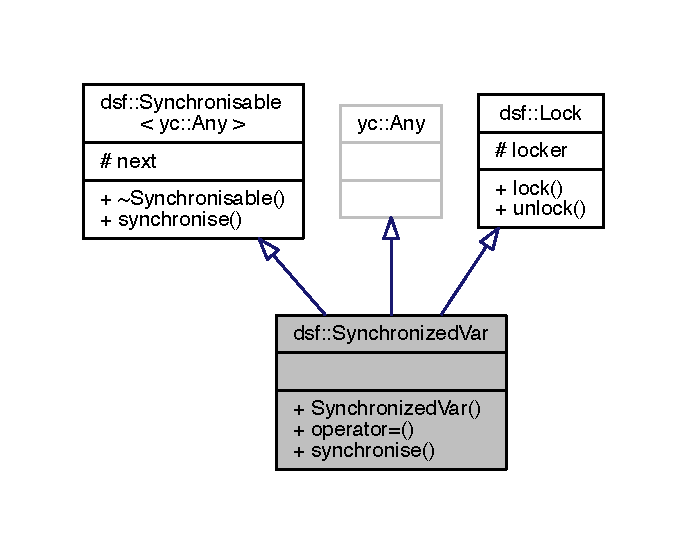
\includegraphics[width=330pt]{classdsf_1_1_synchronized_var__inherit__graph}
\end{center}
\end{figure}
\subsection*{Public Member Functions}
\begin{DoxyCompactItemize}
\item 
{\footnotesize template$<$typename T $>$ }\\\hyperlink{classdsf_1_1_synchronized_var_aada6540bf8bbbf1451834f31aad0962f}{Synchronized\+Var} (T \&\&value)
\item 
{\footnotesize template$<$typename T $>$ }\\void \hyperlink{classdsf_1_1_synchronized_var_a8b72cc04251d677755090bd9b834291c}{operator=} (T \&\&value)
\item 
void \hyperlink{classdsf_1_1_synchronized_var_ac8465a885c4dbb5bc5ca9ad25f42c3ec}{synchronise} () override
\end{DoxyCompactItemize}
\subsection*{Additional Inherited Members}


\subsection{Detailed Description}
A Class which implements \hyperlink{classdsf_1_1_synchronisable}{dsf\+::\+Synchronisable}. 

The purpose of this class is to make thread-\/safe variables for \hyperlink{classdsf_1_1_synchronized_object}{dsf\+::\+Synchronized\+Object} objects. A \hyperlink{classdsf_1_1_synchronized_var}{dsf\+::\+Synchronized\+Var} object has two states -\/ “current” and “next”. The “current” is for read operation, and the “next” is for write operation. The function “synchronise” signs “next” to “current”.\hypertarget{classdsf_1_1_synchronized_var_Example}{}\subsection{Example}\label{classdsf_1_1_synchronized_var_Example}

\begin{DoxyCode}
\hyperlink{classdsf_1_1_synchronized_var}{dsf::SynchronizedVar} myInt;
myInt = int(8); \textcolor{comment}{// value == NULL, next == 8}
myInt.synchronize(); \textcolor{comment}{// value == 8, next == 8}
std::cout << myInt.to<\textcolor{keywordtype}{int}>() << std::endl; \textcolor{comment}{// output 8}
myInt = int(9); \textcolor{comment}{// value == 8, next == 9}
std::cout << myInt.to<\textcolor{keywordtype}{int}>() << std::endl; \textcolor{comment}{// output 8}
myInt.synchronize(); \textcolor{comment}{// value == 9, next == 9}
std::cout << myInt.to<\textcolor{keywordtype}{int}>() << std::endl; \textcolor{comment}{// output 9}
\end{DoxyCode}
 

\subsection{Constructor \& Destructor Documentation}
\hypertarget{classdsf_1_1_synchronized_var_aada6540bf8bbbf1451834f31aad0962f}{}\index{dsf\+::\+Synchronized\+Var@{dsf\+::\+Synchronized\+Var}!Synchronized\+Var@{Synchronized\+Var}}
\index{Synchronized\+Var@{Synchronized\+Var}!dsf\+::\+Synchronized\+Var@{dsf\+::\+Synchronized\+Var}}
\subsubsection[{Synchronized\+Var}]{\setlength{\rightskip}{0pt plus 5cm}template$<$typename T $>$ dsf\+::\+Synchronized\+Var\+::\+Synchronized\+Var (
\begin{DoxyParamCaption}
\item[{T \&\&}]{value}
\end{DoxyParamCaption}
)}\label{classdsf_1_1_synchronized_var_aada6540bf8bbbf1451834f31aad0962f}
The value of \char`\"{}current\char`\"{} and the value of \char`\"{}next\char`\"{} is initialized as \char`\"{}value\char`\"{}. 

\subsection{Member Function Documentation}
\hypertarget{classdsf_1_1_synchronized_var_a8b72cc04251d677755090bd9b834291c}{}\index{dsf\+::\+Synchronized\+Var@{dsf\+::\+Synchronized\+Var}!operator=@{operator=}}
\index{operator=@{operator=}!dsf\+::\+Synchronized\+Var@{dsf\+::\+Synchronized\+Var}}
\subsubsection[{operator=}]{\setlength{\rightskip}{0pt plus 5cm}template$<$typename T $>$ void dsf\+::\+Synchronized\+Var\+::operator= (
\begin{DoxyParamCaption}
\item[{T \&\&}]{value}
\end{DoxyParamCaption}
)}\label{classdsf_1_1_synchronized_var_a8b72cc04251d677755090bd9b834291c}
Signs a value to \char`\"{}next\char`\"{}. 

Here is the call graph for this function\+:\nopagebreak
\begin{figure}[H]
\begin{center}
\leavevmode
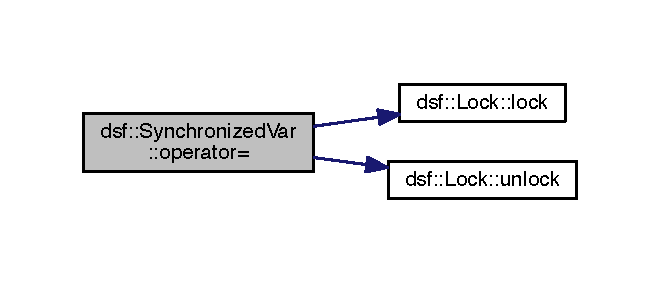
\includegraphics[width=317pt]{classdsf_1_1_synchronized_var_a8b72cc04251d677755090bd9b834291c_cgraph}
\end{center}
\end{figure}


\hypertarget{classdsf_1_1_synchronized_var_ac8465a885c4dbb5bc5ca9ad25f42c3ec}{}\index{dsf\+::\+Synchronized\+Var@{dsf\+::\+Synchronized\+Var}!synchronise@{synchronise}}
\index{synchronise@{synchronise}!dsf\+::\+Synchronized\+Var@{dsf\+::\+Synchronized\+Var}}
\subsubsection[{synchronise}]{\setlength{\rightskip}{0pt plus 5cm}void dsf\+::\+Synchronized\+Var\+::synchronise (
\begin{DoxyParamCaption}
{}
\end{DoxyParamCaption}
)\hspace{0.3cm}{\ttfamily [override]}, {\ttfamily [virtual]}}\label{classdsf_1_1_synchronized_var_ac8465a885c4dbb5bc5ca9ad25f42c3ec}
Signs current value to next value. 

Implements \hyperlink{classdsf_1_1_synchronisable_a225f9a5f6cb47d73e1ea4d788bbfcaaa}{dsf\+::\+Synchronisable$<$ yc\+::\+Any $>$}.



The documentation for this class was generated from the following file\+:\begin{DoxyCompactItemize}
\item 
/\+Users/yuchen/\+Repositories/\+Dual\+State\+Framework/dsf/include/dsf/\hyperlink{_synchronized_var_8h}{Synchronized\+Var.\+h}\end{DoxyCompactItemize}

\hypertarget{classdsf_1_1_task}{}\section{dsf\+:\+:Task Class Reference}
\label{classdsf_1_1_task}\index{dsf\+::\+Task@{dsf\+::\+Task}}


Class \hyperlink{classdsf_1_1_task}{Task}.  




{\ttfamily \#include $<$Task.\+h$>$}

\subsection*{Public Member Functions}
\begin{DoxyCompactItemize}
\item 
\hyperlink{classdsf_1_1_task_afa460a63f94f30df36df5661de1dbe1a}{Task} (\hyperlink{classdsf_1_1_synchronized_object}{Synchronized\+Object} $\ast$\hyperlink{classdsf_1_1_task_a36c485fbeb9c2330f5637b9d625cf01a}{to}, \hyperlink{classdsf_1_1_synchronized_object}{Synchronized\+Object} $\ast$\hyperlink{classdsf_1_1_task_afc1faf30dab0d57501dfdcb4ef7b5450}{from}, \hyperlink{namespacedsf_aa16e735f29587f4485b56fc46746f7a9}{Task\+Function} $\ast$\hyperlink{classdsf_1_1_task_a681617cab34fbae641c5b0cf4be46659}{task\+Function}, \hyperlink{namespacedsf_abe4bf68433935a81c31a5ada9b17663a}{Task\+Argument} $\ast$\hyperlink{classdsf_1_1_task_a8a095d8a36668f6500d4df8c24dbef8d}{task\+Argument})
\item 
\hyperlink{classdsf_1_1_task_a617ffc1b2f418f061fbc168d74ed5a55}{$\sim$\+Task} ()
\end{DoxyCompactItemize}
\subsection*{Public Attributes}
\begin{DoxyCompactItemize}
\item 
\hyperlink{classdsf_1_1_synchronized_object}{Synchronized\+Object} $\ast$ \hyperlink{classdsf_1_1_task_a36c485fbeb9c2330f5637b9d625cf01a}{to}
\item 
\hyperlink{classdsf_1_1_synchronized_object}{Synchronized\+Object} $\ast$ \hyperlink{classdsf_1_1_task_afc1faf30dab0d57501dfdcb4ef7b5450}{from}
\item 
\hyperlink{namespacedsf_aa16e735f29587f4485b56fc46746f7a9}{Task\+Function} $\ast$ \hyperlink{classdsf_1_1_task_a681617cab34fbae641c5b0cf4be46659}{task\+Function}
\item 
\hyperlink{namespacedsf_abe4bf68433935a81c31a5ada9b17663a}{Task\+Argument} $\ast$ \hyperlink{classdsf_1_1_task_a8a095d8a36668f6500d4df8c24dbef8d}{task\+Argument}
\end{DoxyCompactItemize}


\subsection{Detailed Description}
Class \hyperlink{classdsf_1_1_task}{Task}. 

This class have four members\+: from, to, function, and arguments, where \char`\"{}from\char`\"{} is a \hyperlink{classdsf_1_1_synchronized_object}{dsf\+::\+Synchronized\+Object} object who sent message to you. 

\subsection{Constructor \& Destructor Documentation}
\hypertarget{classdsf_1_1_task_afa460a63f94f30df36df5661de1dbe1a}{}\index{dsf\+::\+Task@{dsf\+::\+Task}!Task@{Task}}
\index{Task@{Task}!dsf\+::\+Task@{dsf\+::\+Task}}
\subsubsection[{Task}]{\setlength{\rightskip}{0pt plus 5cm}dsf\+::\+Task\+::\+Task (
\begin{DoxyParamCaption}
\item[{{\bf Synchronized\+Object} $\ast$}]{to, }
\item[{{\bf Synchronized\+Object} $\ast$}]{from, }
\item[{{\bf Task\+Function} $\ast$}]{task\+Function, }
\item[{{\bf Task\+Argument} $\ast$}]{task\+Argument}
\end{DoxyParamCaption}
)\hspace{0.3cm}{\ttfamily [explicit]}}\label{classdsf_1_1_task_afa460a63f94f30df36df5661de1dbe1a}
\hypertarget{classdsf_1_1_task_a617ffc1b2f418f061fbc168d74ed5a55}{}\index{dsf\+::\+Task@{dsf\+::\+Task}!````~Task@{$\sim$\+Task}}
\index{````~Task@{$\sim$\+Task}!dsf\+::\+Task@{dsf\+::\+Task}}
\subsubsection[{$\sim$\+Task}]{\setlength{\rightskip}{0pt plus 5cm}dsf\+::\+Task\+::$\sim$\+Task (
\begin{DoxyParamCaption}
{}
\end{DoxyParamCaption}
)}\label{classdsf_1_1_task_a617ffc1b2f418f061fbc168d74ed5a55}


\subsection{Member Data Documentation}
\hypertarget{classdsf_1_1_task_afc1faf30dab0d57501dfdcb4ef7b5450}{}\index{dsf\+::\+Task@{dsf\+::\+Task}!from@{from}}
\index{from@{from}!dsf\+::\+Task@{dsf\+::\+Task}}
\subsubsection[{from}]{\setlength{\rightskip}{0pt plus 5cm}{\bf Synchronized\+Object}$\ast$ dsf\+::\+Task\+::from}\label{classdsf_1_1_task_afc1faf30dab0d57501dfdcb4ef7b5450}
Where the message is sent from. \hypertarget{classdsf_1_1_task_a8a095d8a36668f6500d4df8c24dbef8d}{}\index{dsf\+::\+Task@{dsf\+::\+Task}!task\+Argument@{task\+Argument}}
\index{task\+Argument@{task\+Argument}!dsf\+::\+Task@{dsf\+::\+Task}}
\subsubsection[{task\+Argument}]{\setlength{\rightskip}{0pt plus 5cm}{\bf Task\+Argument}$\ast$ dsf\+::\+Task\+::task\+Argument}\label{classdsf_1_1_task_a8a095d8a36668f6500d4df8c24dbef8d}
The arguments for the function pointer. \hypertarget{classdsf_1_1_task_a681617cab34fbae641c5b0cf4be46659}{}\index{dsf\+::\+Task@{dsf\+::\+Task}!task\+Function@{task\+Function}}
\index{task\+Function@{task\+Function}!dsf\+::\+Task@{dsf\+::\+Task}}
\subsubsection[{task\+Function}]{\setlength{\rightskip}{0pt plus 5cm}{\bf Task\+Function}$\ast$ dsf\+::\+Task\+::task\+Function}\label{classdsf_1_1_task_a681617cab34fbae641c5b0cf4be46659}
The function pointer. \hypertarget{classdsf_1_1_task_a36c485fbeb9c2330f5637b9d625cf01a}{}\index{dsf\+::\+Task@{dsf\+::\+Task}!to@{to}}
\index{to@{to}!dsf\+::\+Task@{dsf\+::\+Task}}
\subsubsection[{to}]{\setlength{\rightskip}{0pt plus 5cm}{\bf Synchronized\+Object}$\ast$ dsf\+::\+Task\+::to}\label{classdsf_1_1_task_a36c485fbeb9c2330f5637b9d625cf01a}
Where the message is sent to. 

The documentation for this class was generated from the following file\+:\begin{DoxyCompactItemize}
\item 
Task.\+h\end{DoxyCompactItemize}

\hypertarget{classdsf_1_1_task_box}{}\section{dsf\+:\+:Task\+Box Class Reference}
\label{classdsf_1_1_task_box}\index{dsf\+::\+Task\+Box@{dsf\+::\+Task\+Box}}


A \hyperlink{classdsf_1_1_task}{dsf\+::\+Task} queue.  




{\ttfamily \#include $<$Task\+Box.\+h$>$}



Inheritance diagram for dsf\+:\+:Task\+Box\+:\nopagebreak
\begin{figure}[H]
\begin{center}
\leavevmode
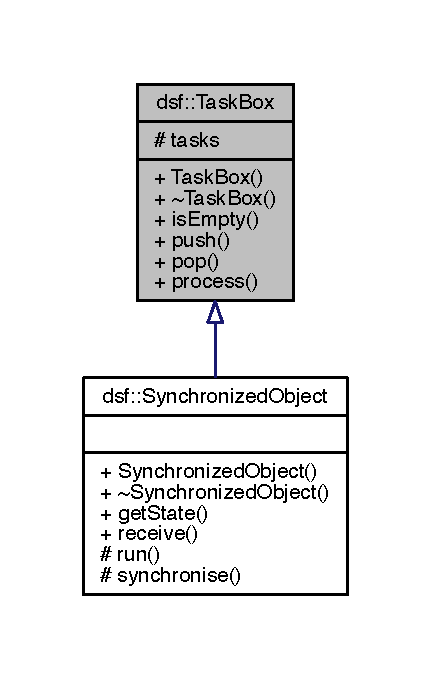
\includegraphics[width=207pt]{classdsf_1_1_task_box__inherit__graph}
\end{center}
\end{figure}
\subsection*{Public Member Functions}
\begin{DoxyCompactItemize}
\item 
\hyperlink{classdsf_1_1_task_box_a931c925e0a4956ee6bc1674f43ecc0a0}{Task\+Box} ()
\item 
virtual \hyperlink{classdsf_1_1_task_box_a20684b560a76fc97dd8e3f879ea240df}{$\sim$\+Task\+Box} ()
\item 
bool \hyperlink{classdsf_1_1_task_box_a7e67fd9b7104d24cb4be54f6a48eb8c9}{is\+Empty} ()
\item 
void \hyperlink{classdsf_1_1_task_box_a0ec4e52a625fae00e05b072d6434eef1}{push} (\hyperlink{classdsf_1_1_task}{Task} $\ast$task)
\item 
\hyperlink{classdsf_1_1_task}{Task} $\ast$ \hyperlink{classdsf_1_1_task_box_a656f4778edd42d43ff7516de3fa528ef}{pop} ()
\item 
void \hyperlink{classdsf_1_1_task_box_ad35070ac305146aaa4073b2078d9209e}{process} ()
\end{DoxyCompactItemize}
\subsection*{Protected Attributes}
\begin{DoxyCompactItemize}
\item 
std\+::vector$<$ \hyperlink{classdsf_1_1_task}{Task} $\ast$ $>$ $\ast$ \hyperlink{classdsf_1_1_task_box_ae13d0d245cacbf7f4019f7ff5486aa79}{tasks}
\end{DoxyCompactItemize}


\subsection{Detailed Description}
A \hyperlink{classdsf_1_1_task}{dsf\+::\+Task} queue. 

The \hyperlink{classdsf_1_1_task_box}{dsf\+::\+Task\+Box} contains a list of def\+::\+Task objects. It provides essential methods to control the list such as “push”, “pop”, and “is\+Empty”. 

\subsection{Constructor \& Destructor Documentation}
\hypertarget{classdsf_1_1_task_box_a931c925e0a4956ee6bc1674f43ecc0a0}{}\index{dsf\+::\+Task\+Box@{dsf\+::\+Task\+Box}!Task\+Box@{Task\+Box}}
\index{Task\+Box@{Task\+Box}!dsf\+::\+Task\+Box@{dsf\+::\+Task\+Box}}
\subsubsection[{Task\+Box}]{\setlength{\rightskip}{0pt plus 5cm}dsf\+::\+Task\+Box\+::\+Task\+Box (
\begin{DoxyParamCaption}
{}
\end{DoxyParamCaption}
)}\label{classdsf_1_1_task_box_a931c925e0a4956ee6bc1674f43ecc0a0}
\hypertarget{classdsf_1_1_task_box_a20684b560a76fc97dd8e3f879ea240df}{}\index{dsf\+::\+Task\+Box@{dsf\+::\+Task\+Box}!````~Task\+Box@{$\sim$\+Task\+Box}}
\index{````~Task\+Box@{$\sim$\+Task\+Box}!dsf\+::\+Task\+Box@{dsf\+::\+Task\+Box}}
\subsubsection[{$\sim$\+Task\+Box}]{\setlength{\rightskip}{0pt plus 5cm}virtual dsf\+::\+Task\+Box\+::$\sim$\+Task\+Box (
\begin{DoxyParamCaption}
{}
\end{DoxyParamCaption}
)\hspace{0.3cm}{\ttfamily [virtual]}}\label{classdsf_1_1_task_box_a20684b560a76fc97dd8e3f879ea240df}


\subsection{Member Function Documentation}
\hypertarget{classdsf_1_1_task_box_a7e67fd9b7104d24cb4be54f6a48eb8c9}{}\index{dsf\+::\+Task\+Box@{dsf\+::\+Task\+Box}!is\+Empty@{is\+Empty}}
\index{is\+Empty@{is\+Empty}!dsf\+::\+Task\+Box@{dsf\+::\+Task\+Box}}
\subsubsection[{is\+Empty}]{\setlength{\rightskip}{0pt plus 5cm}bool dsf\+::\+Task\+Box\+::is\+Empty (
\begin{DoxyParamCaption}
{}
\end{DoxyParamCaption}
)}\label{classdsf_1_1_task_box_a7e67fd9b7104d24cb4be54f6a48eb8c9}
Checks wheather the queue is empty or not. \hypertarget{classdsf_1_1_task_box_a656f4778edd42d43ff7516de3fa528ef}{}\index{dsf\+::\+Task\+Box@{dsf\+::\+Task\+Box}!pop@{pop}}
\index{pop@{pop}!dsf\+::\+Task\+Box@{dsf\+::\+Task\+Box}}
\subsubsection[{pop}]{\setlength{\rightskip}{0pt plus 5cm}{\bf Task}$\ast$ dsf\+::\+Task\+Box\+::pop (
\begin{DoxyParamCaption}
{}
\end{DoxyParamCaption}
)}\label{classdsf_1_1_task_box_a656f4778edd42d43ff7516de3fa528ef}
Pops out a task and returns it \hypertarget{classdsf_1_1_task_box_ad35070ac305146aaa4073b2078d9209e}{}\index{dsf\+::\+Task\+Box@{dsf\+::\+Task\+Box}!process@{process}}
\index{process@{process}!dsf\+::\+Task\+Box@{dsf\+::\+Task\+Box}}
\subsubsection[{process}]{\setlength{\rightskip}{0pt plus 5cm}void dsf\+::\+Task\+Box\+::process (
\begin{DoxyParamCaption}
{}
\end{DoxyParamCaption}
)}\label{classdsf_1_1_task_box_ad35070ac305146aaa4073b2078d9209e}
Pops out all tasks in the queue and executes them. \hypertarget{classdsf_1_1_task_box_a0ec4e52a625fae00e05b072d6434eef1}{}\index{dsf\+::\+Task\+Box@{dsf\+::\+Task\+Box}!push@{push}}
\index{push@{push}!dsf\+::\+Task\+Box@{dsf\+::\+Task\+Box}}
\subsubsection[{push}]{\setlength{\rightskip}{0pt plus 5cm}void dsf\+::\+Task\+Box\+::push (
\begin{DoxyParamCaption}
\item[{{\bf Task} $\ast$}]{task}
\end{DoxyParamCaption}
)}\label{classdsf_1_1_task_box_a0ec4e52a625fae00e05b072d6434eef1}
Pushes a task into the queue. 

\subsection{Member Data Documentation}
\hypertarget{classdsf_1_1_task_box_ae13d0d245cacbf7f4019f7ff5486aa79}{}\index{dsf\+::\+Task\+Box@{dsf\+::\+Task\+Box}!tasks@{tasks}}
\index{tasks@{tasks}!dsf\+::\+Task\+Box@{dsf\+::\+Task\+Box}}
\subsubsection[{tasks}]{\setlength{\rightskip}{0pt plus 5cm}std\+::vector$<${\bf Task}$\ast$$>$$\ast$ dsf\+::\+Task\+Box\+::tasks\hspace{0.3cm}{\ttfamily [protected]}}\label{classdsf_1_1_task_box_ae13d0d245cacbf7f4019f7ff5486aa79}
The list of \hyperlink{classdsf_1_1_task}{dsf\+::\+Task}. 

The documentation for this class was generated from the following file\+:\begin{DoxyCompactItemize}
\item 
/\+Users/yuchen/\+Repositories/\+Dual\+State\+Framework/dsf/include/dsf/\hyperlink{_task_box_8h}{Task\+Box.\+h}\end{DoxyCompactItemize}

%--- End generated contents ---

% Index
\backmatter
\newpage
\phantomsection
\clearemptydoublepage
\addcontentsline{toc}{chapter}{Index}
\printindex

\end{document}
